\chapter {Používateľské rozhranie}
V tejto prílohe sa nachádzajú snímky obrazoviek zobrazujúce používateľské rozhranie implementovanej webovej aplikácie.

\begin {figure}[H]
        \centering
        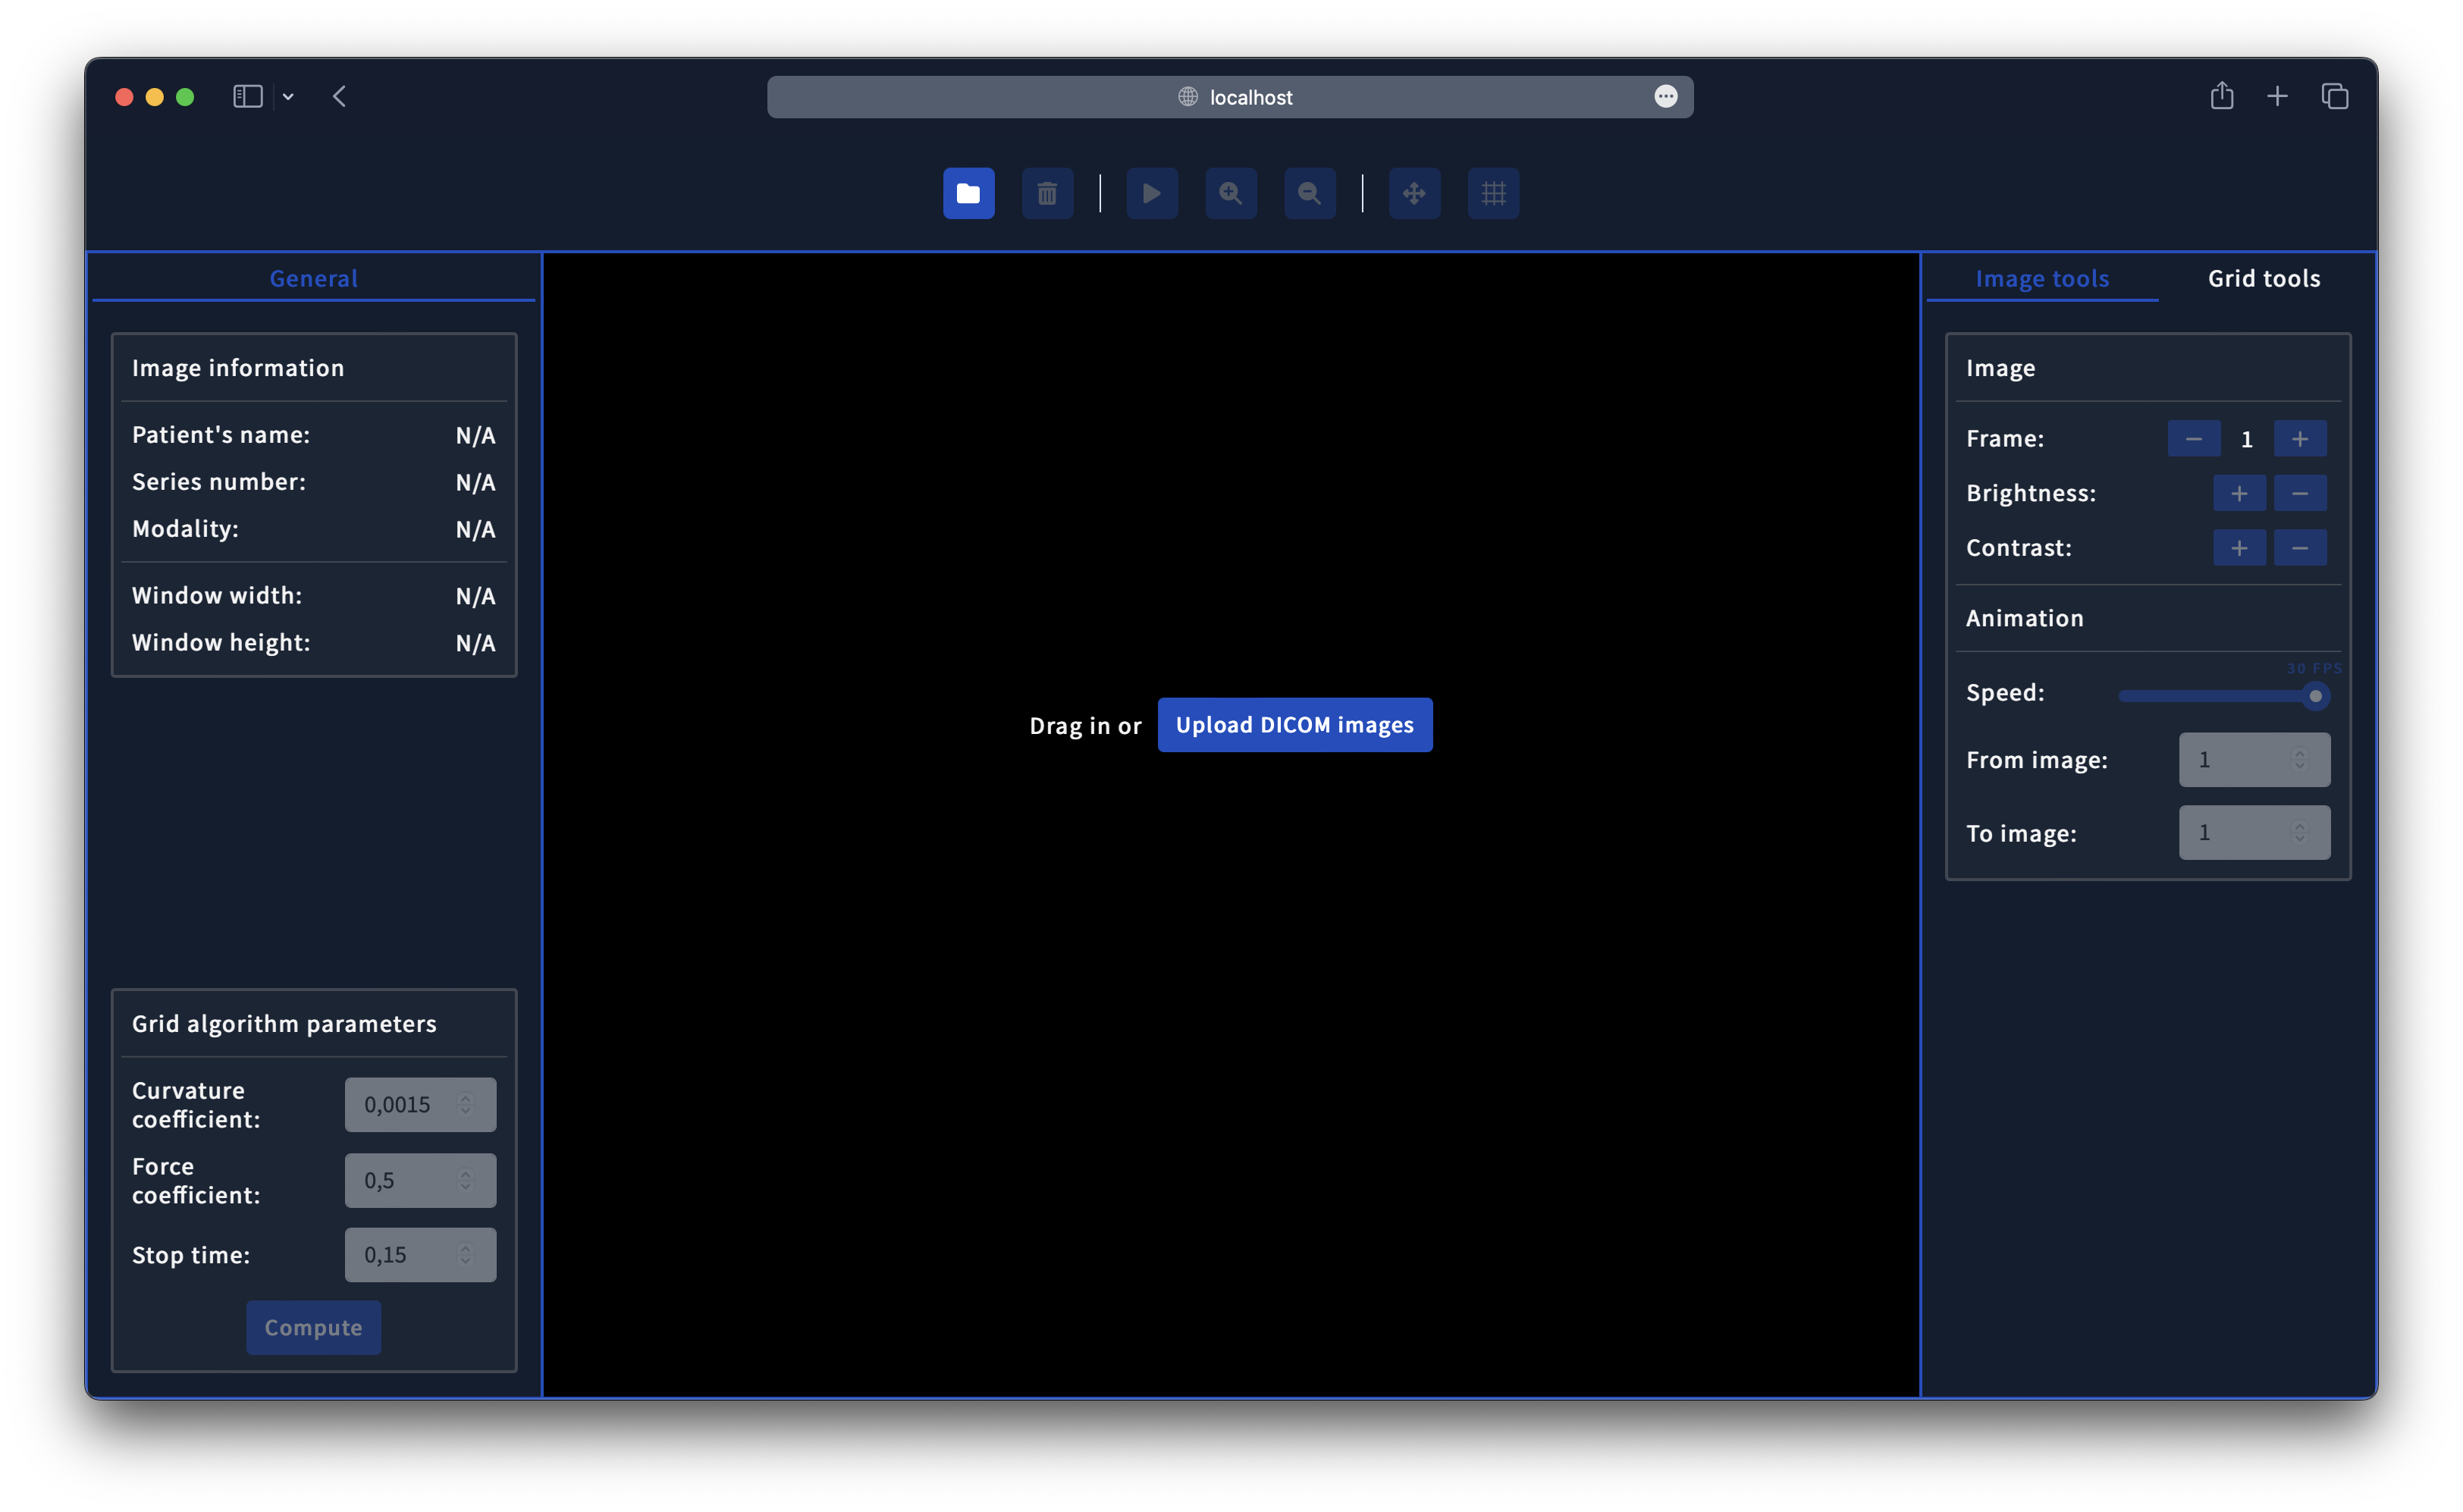
\includegraphics[height=9cm]{media/new_app/initial_state.png}
        \captionsetup{justification=centering}
        \captionof{figure}{Snímka zobrazujúca počiatočný stav aplikácie po jej načítaní.}
\end {figure}

\begin {figure}[H]
        \centering
        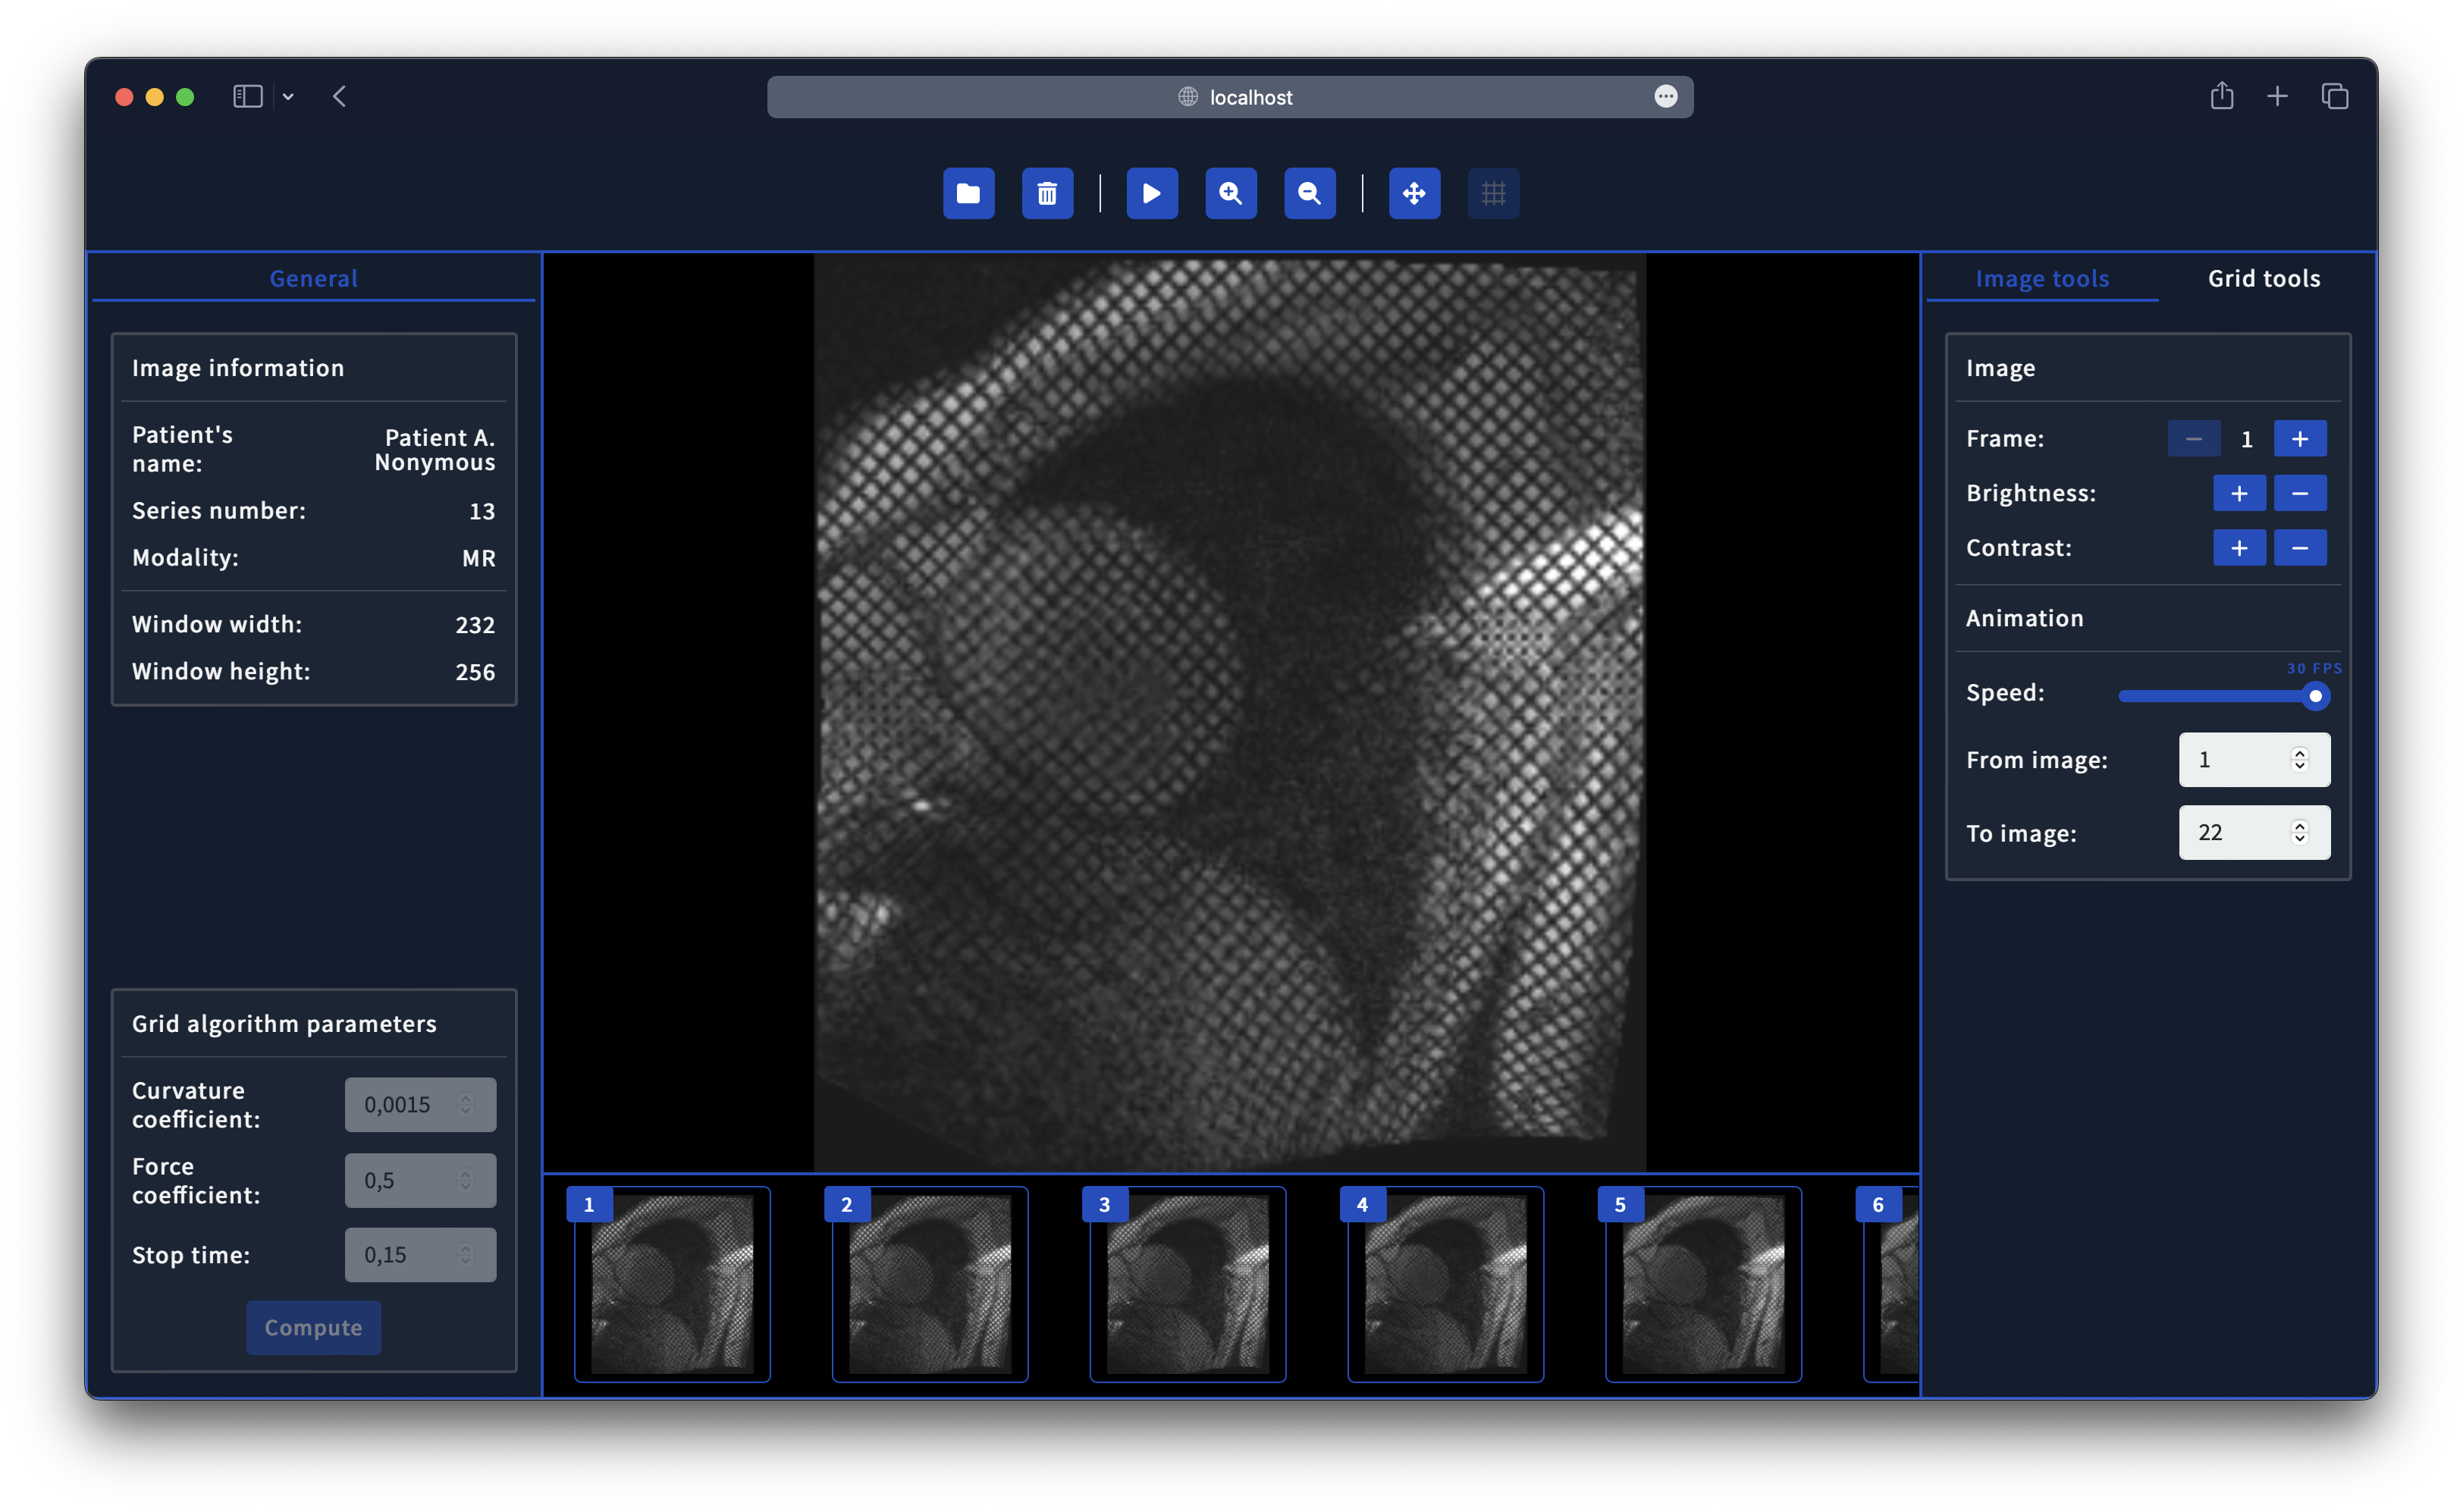
\includegraphics[height=9cm]{media/new_app/state_after_import.png}
        \captionsetup{justification=centering}
        \captionof{figure}{Snímka zobrazujúca stav aplikácie po importovaní DICOM snímiek.}
\end {figure}

\begin {figure}[H]
        \centering
        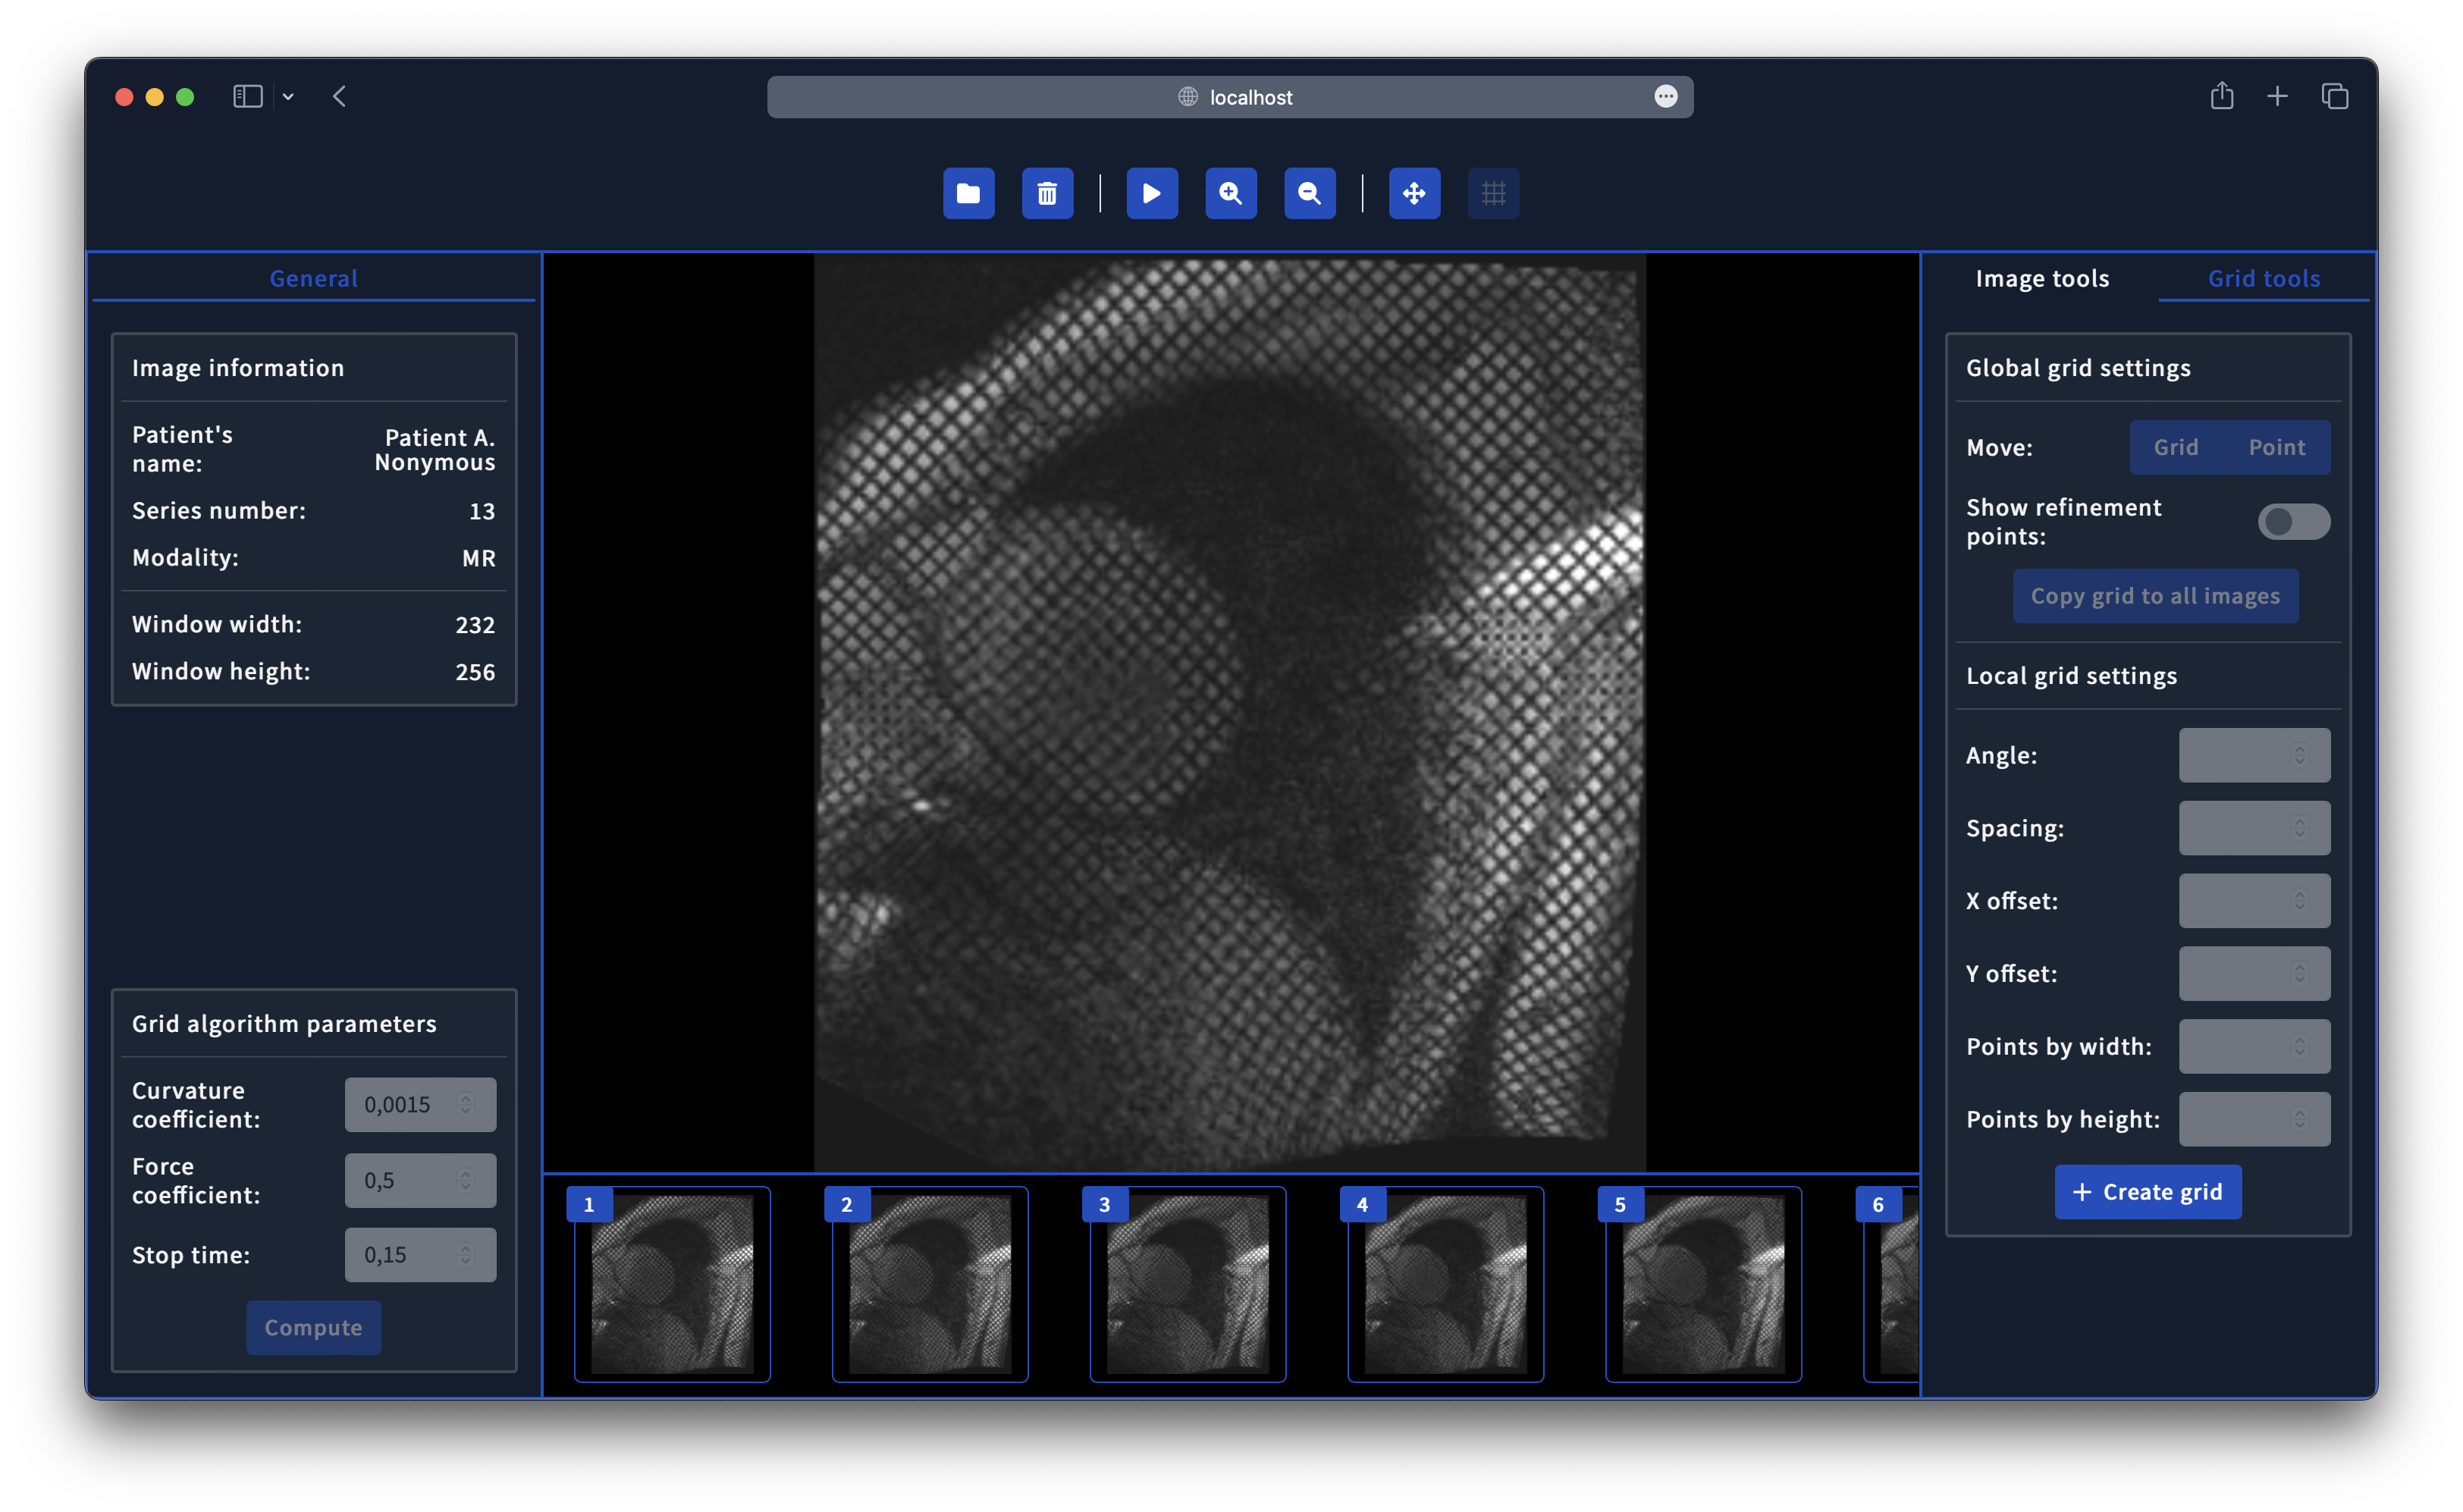
\includegraphics[height=9cm]{media/new_app/grid_tools.png}
        \captionsetup{justification=centering}
        \captionof{figure}{Snímka zobrazujúca kartu \uv{Grid tool} v pravom postrannom paneli.}
\end {figure}

\begin {figure}[H]
        \centering
        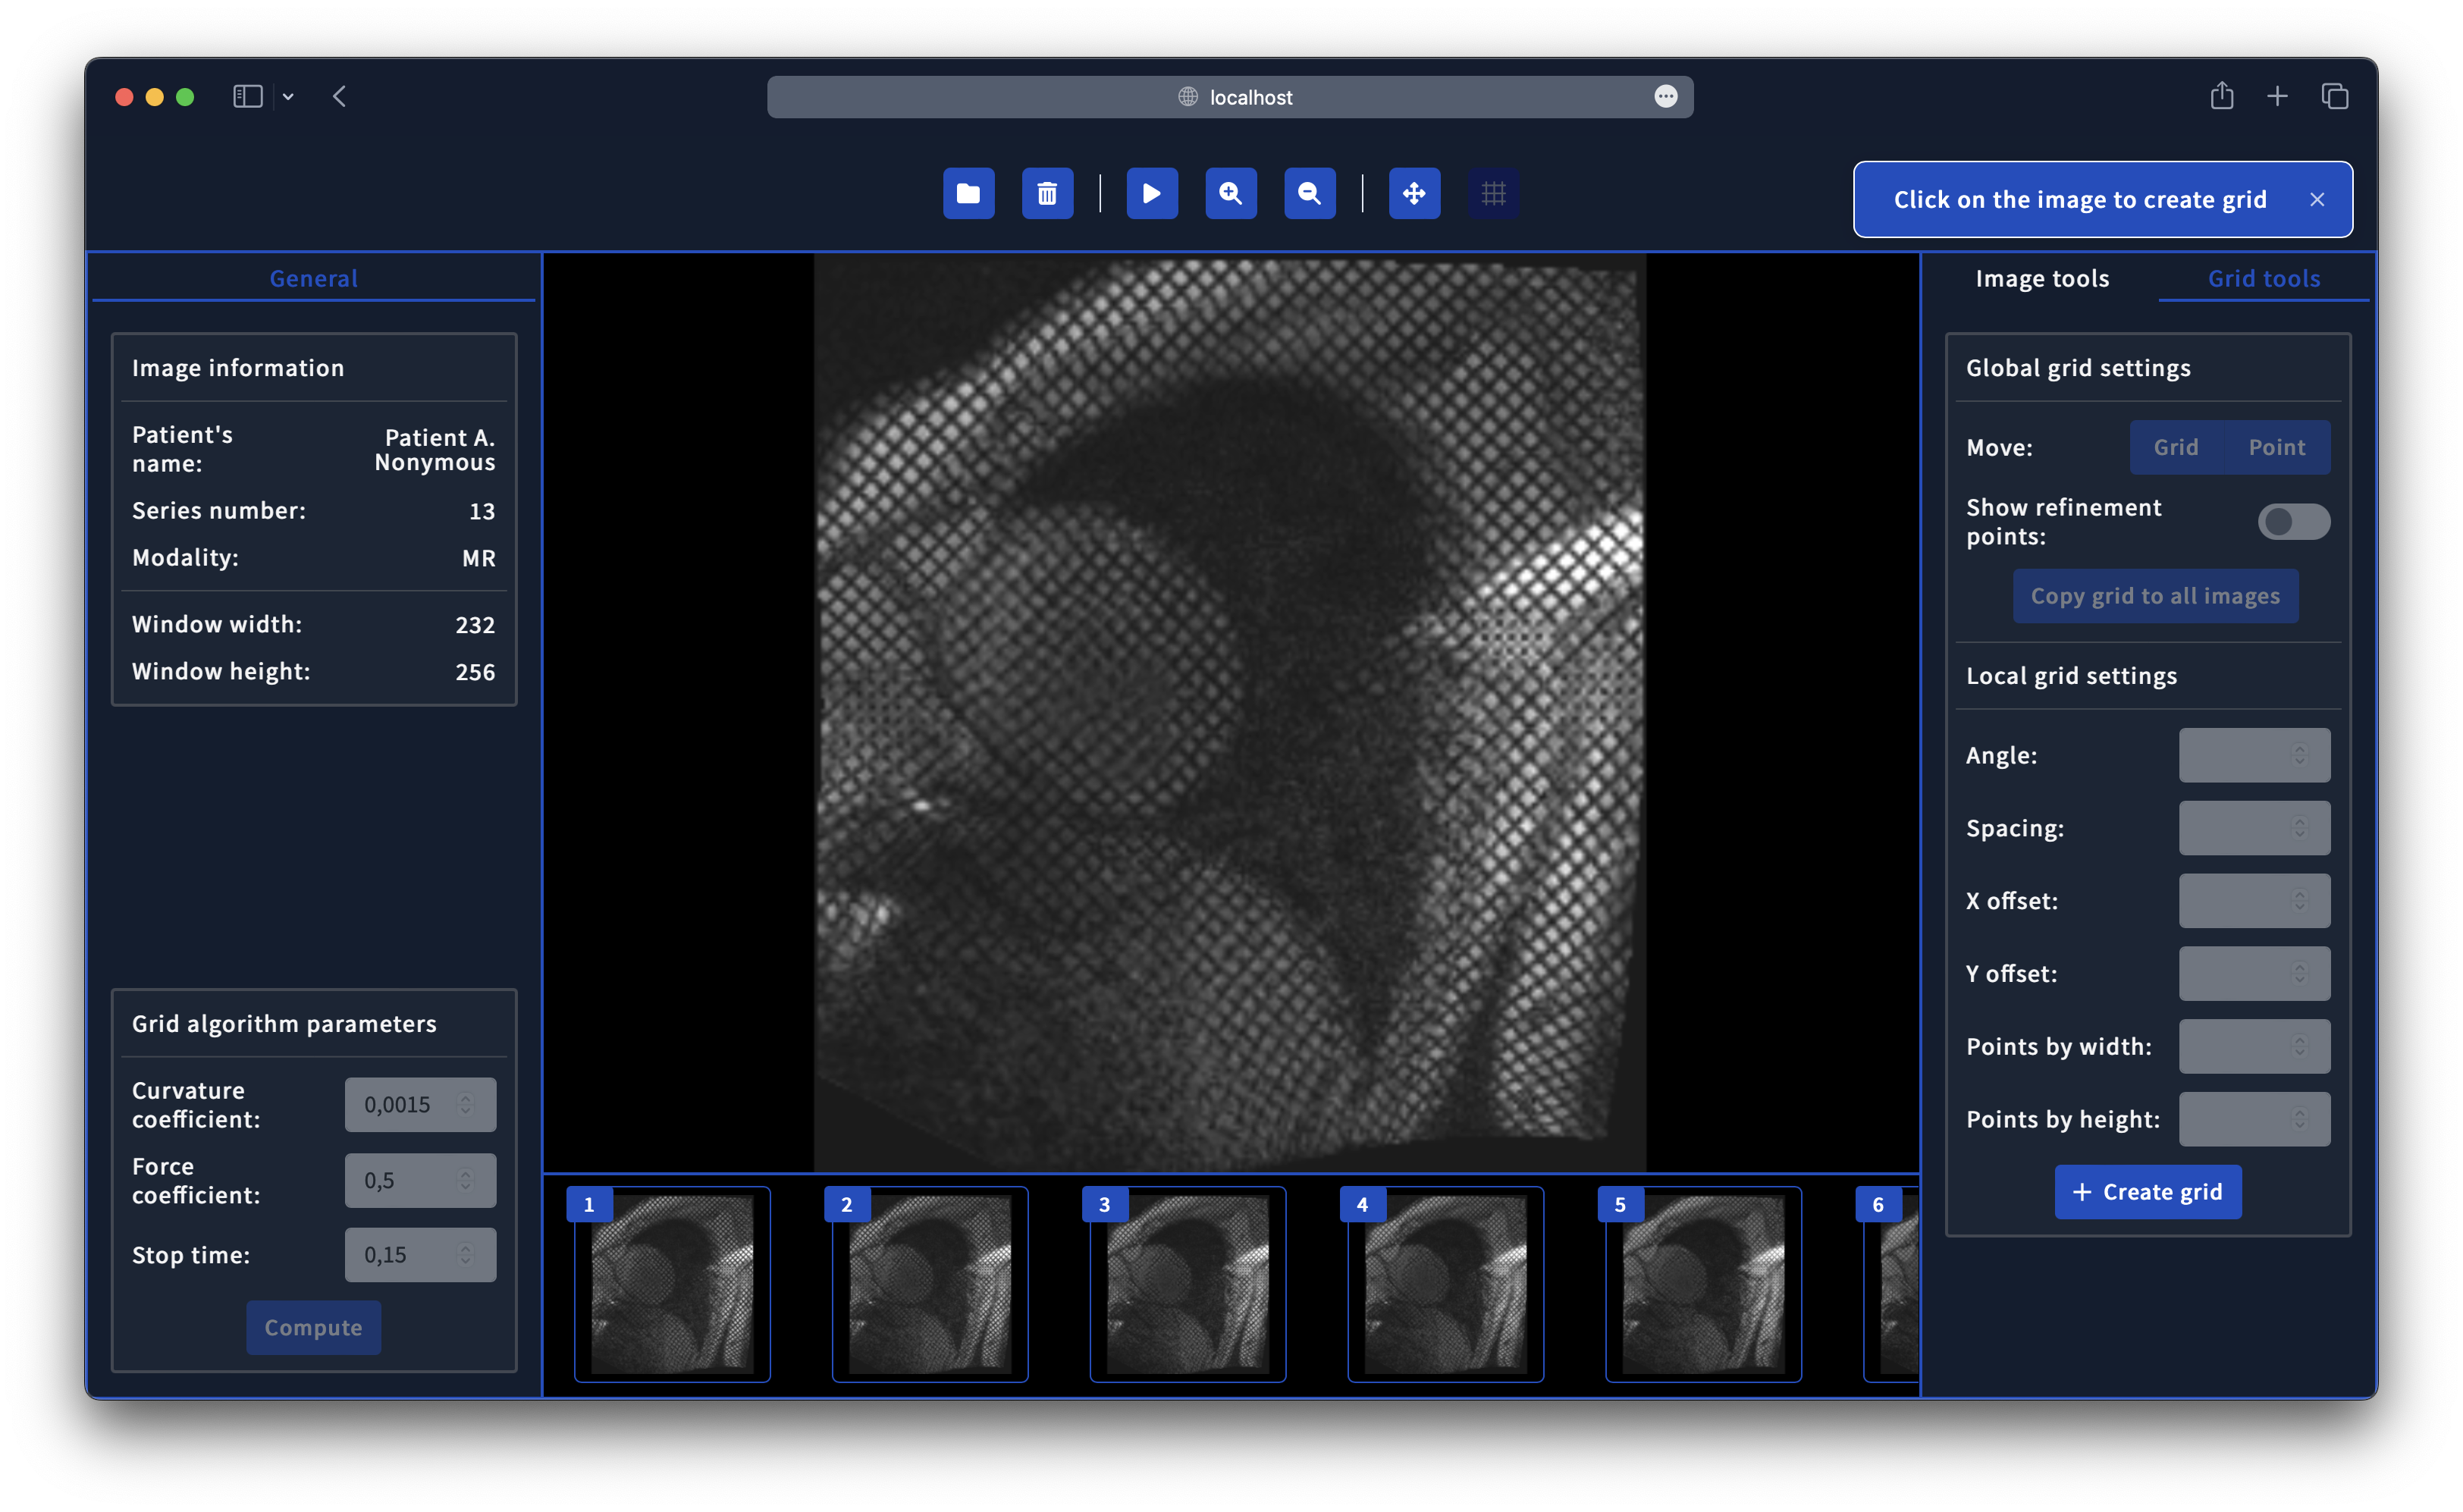
\includegraphics[height=9cm]{media/new_app/notification.png}
        \captionsetup{justification=centering}
        \captionof{figure}{Snímka zobrazujúca notifikáciu aplikácie s krokom pre vytvorenie mriežky.}
\end {figure}

\begin {figure}[H]
        \centering
        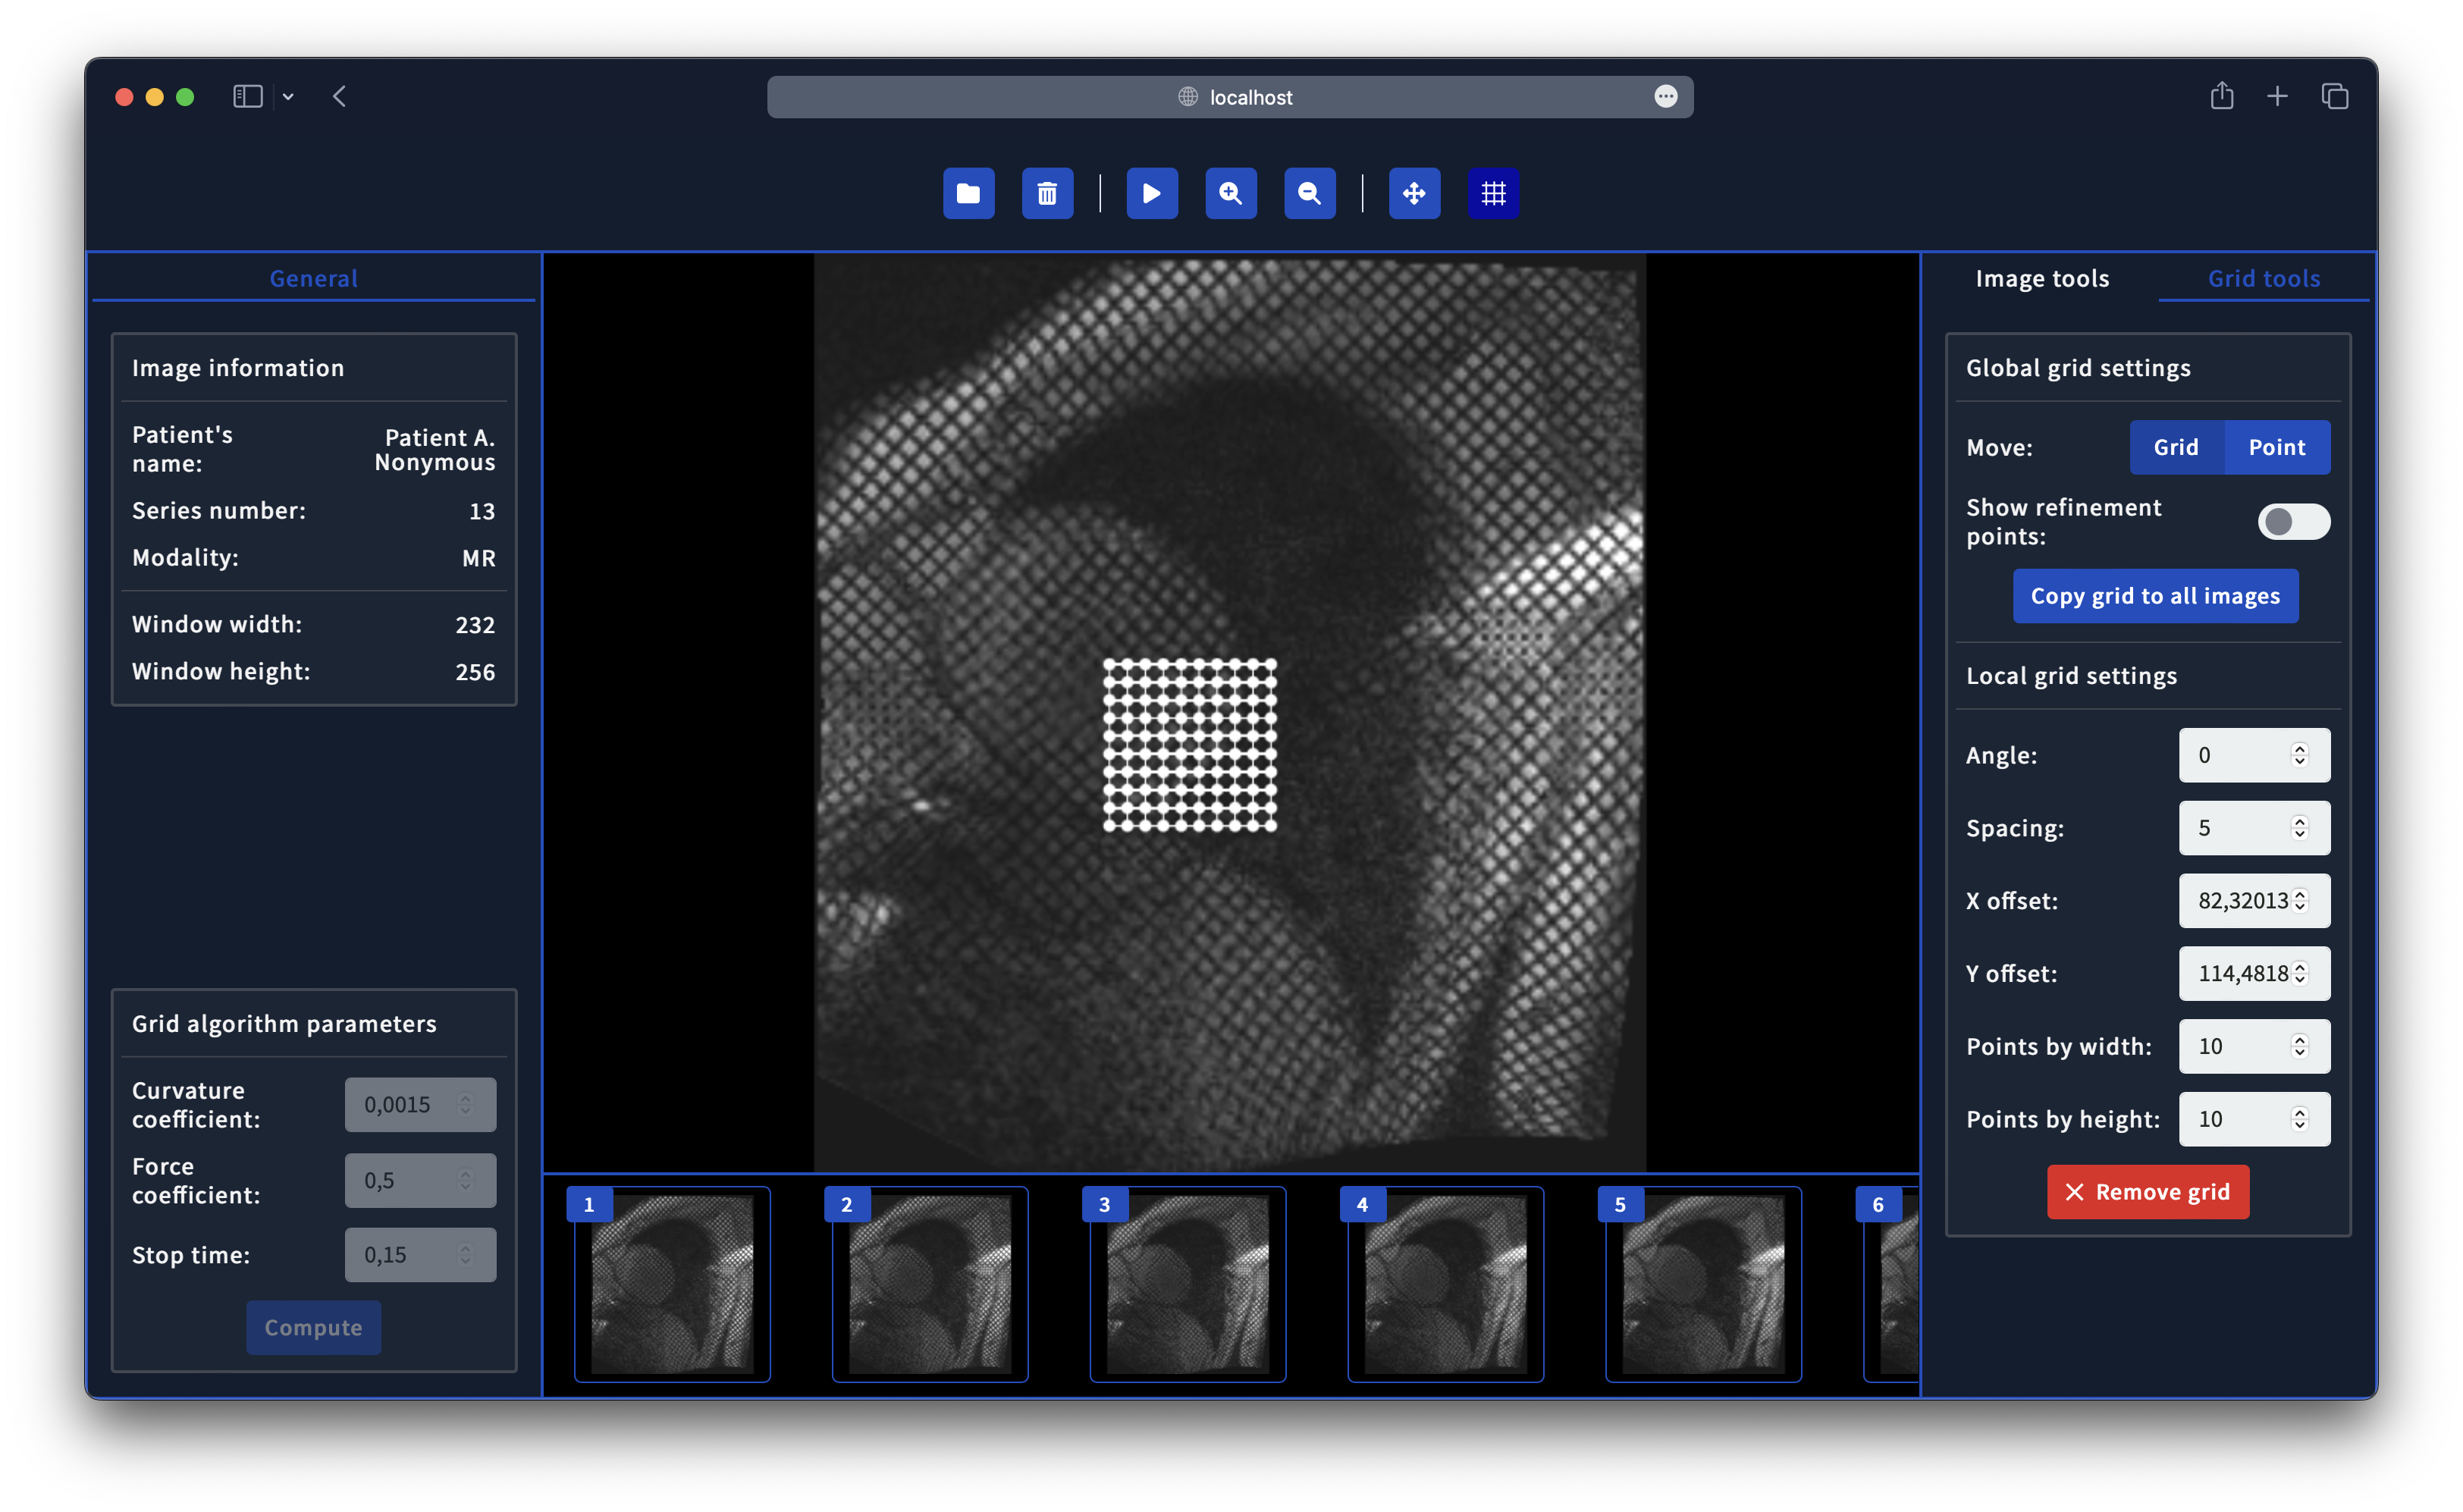
\includegraphics[height=9cm]{media/new_app/grid.png}
        \captionsetup{justification=centering}
        \captionof{figure}{Snímka zobrazujúca vygenerovanú mriežku zobrazenú nad DICOM snímkou.}
\end {figure}

\begin {figure}[H]
        \centering
        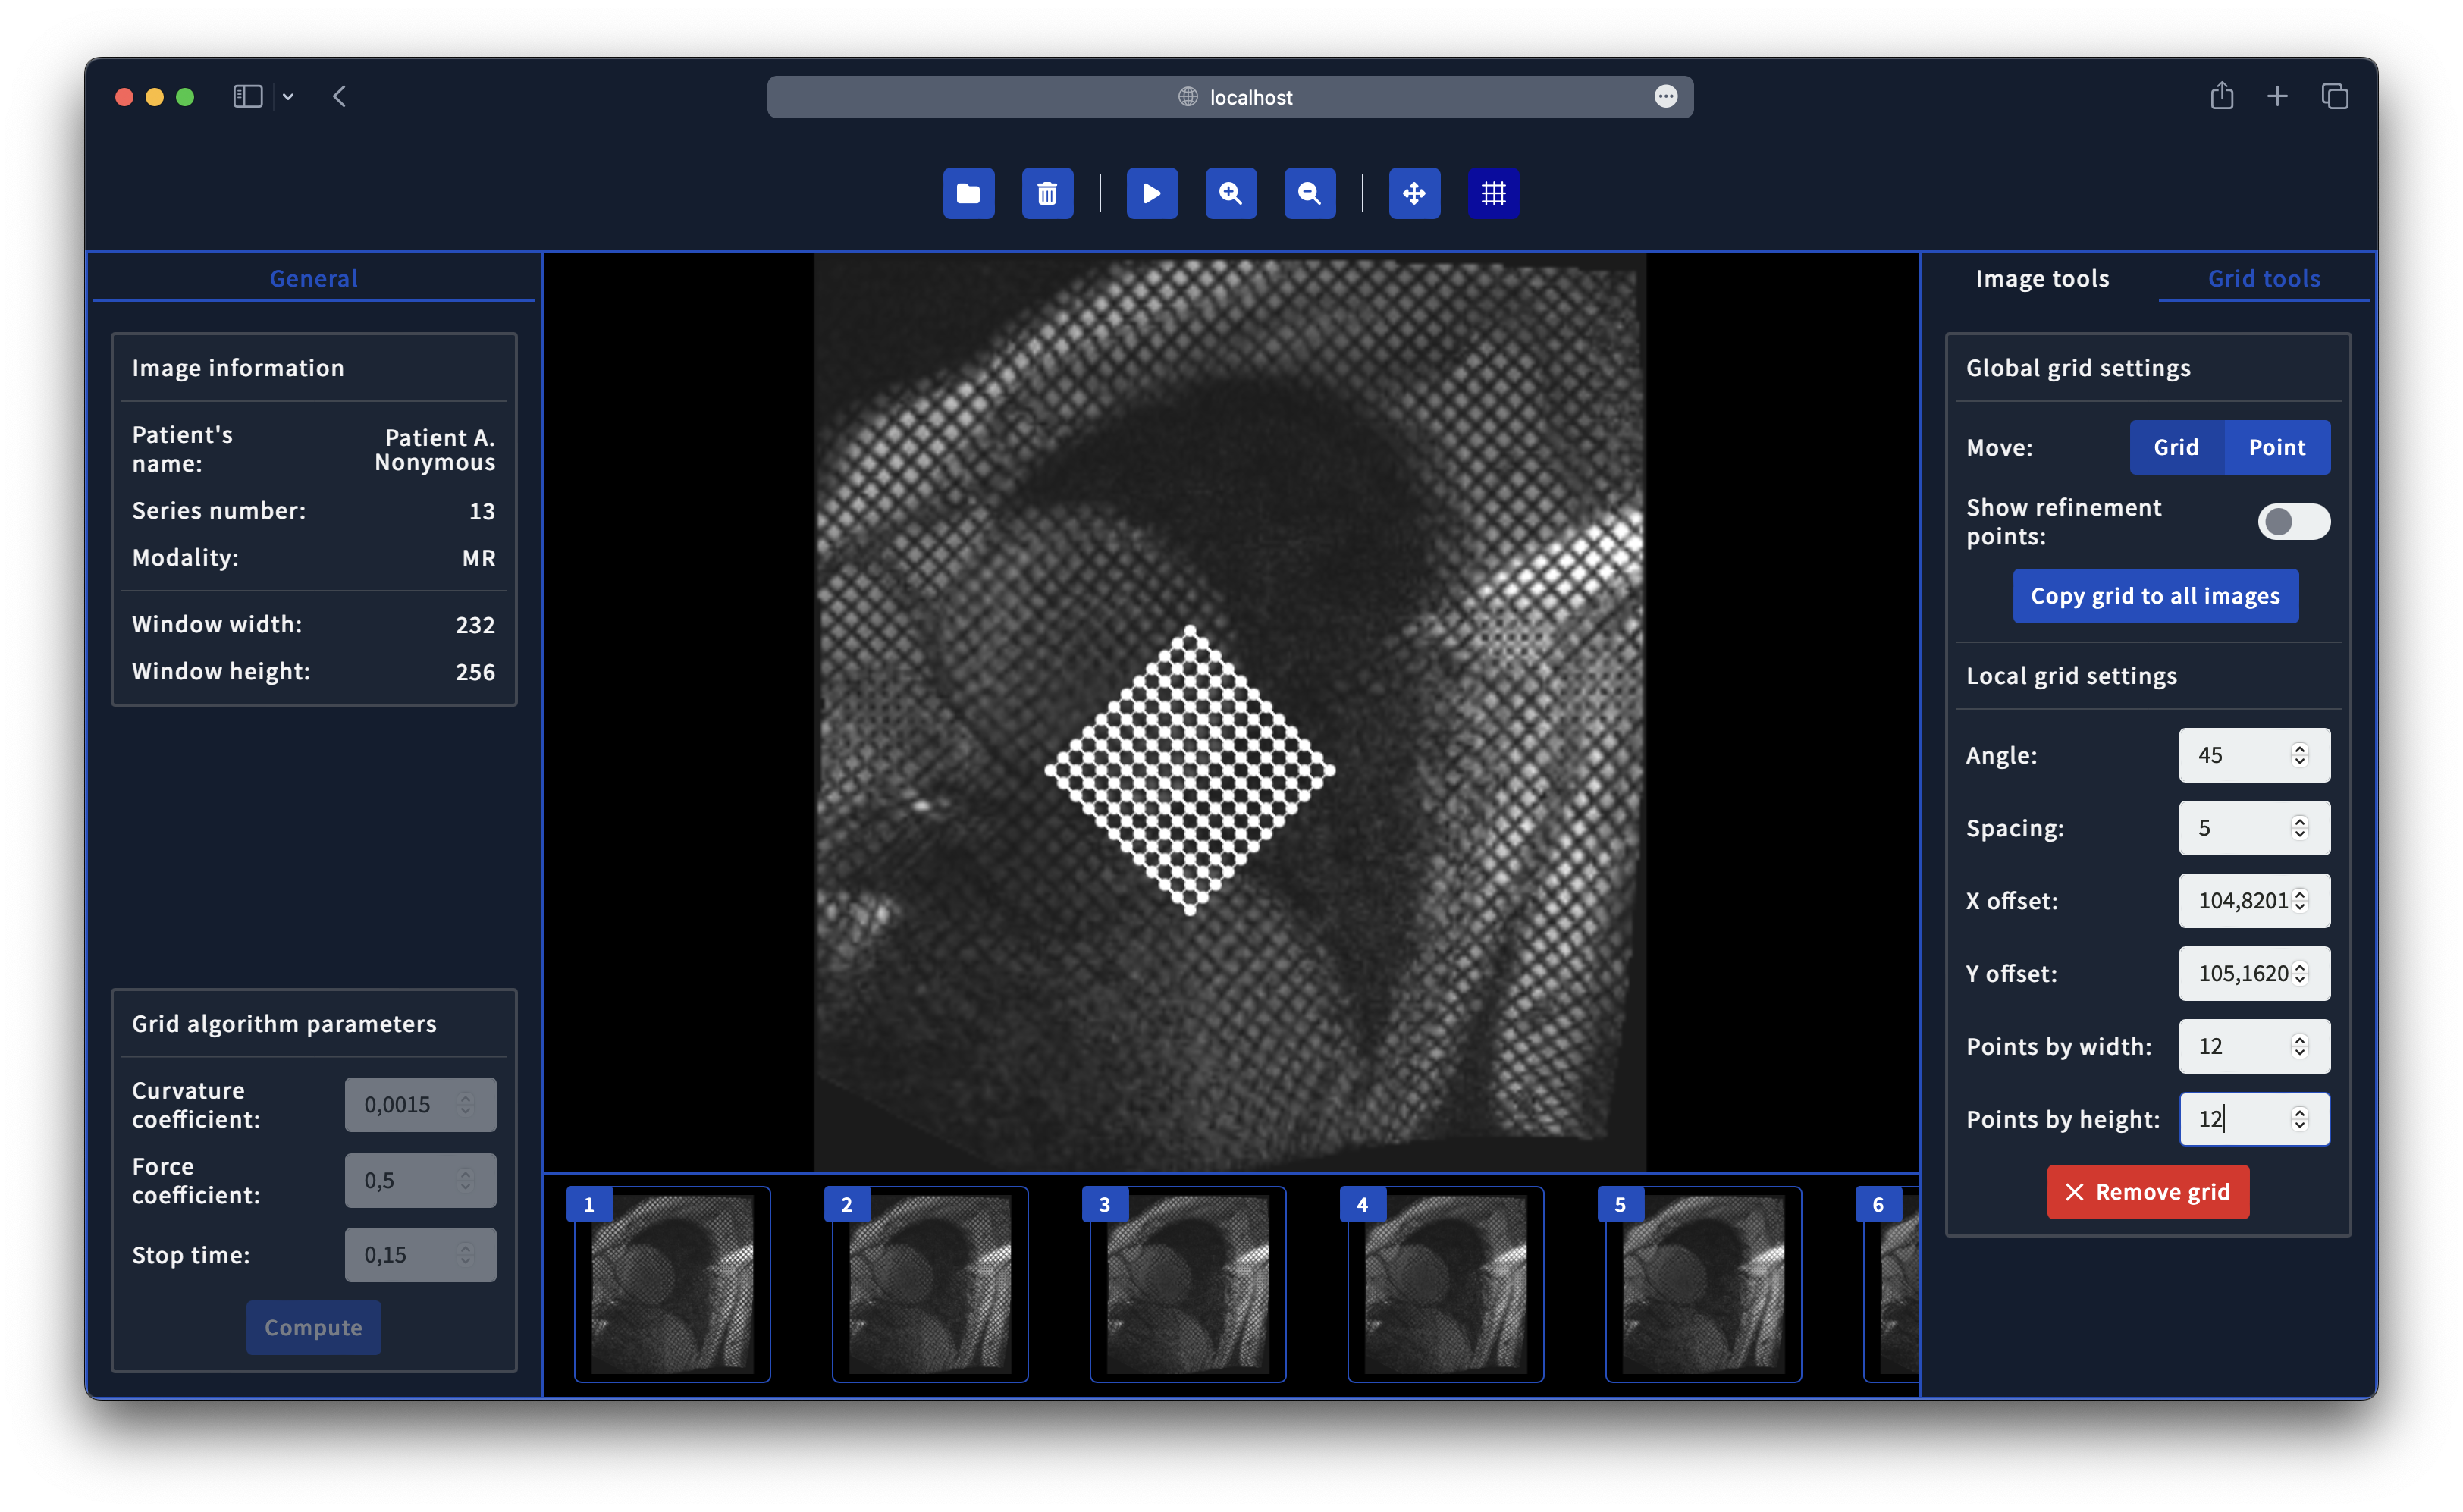
\includegraphics[height=9cm]{media/new_app/grid_modification.png}
        \captionsetup{justification=centering}
        \captionof{figure}{Snímka zobrazujúca zmenu štruktúry mriežky na základe zmenených parametrov.}
\end {figure}

\begin {figure}[H]
        \centering
        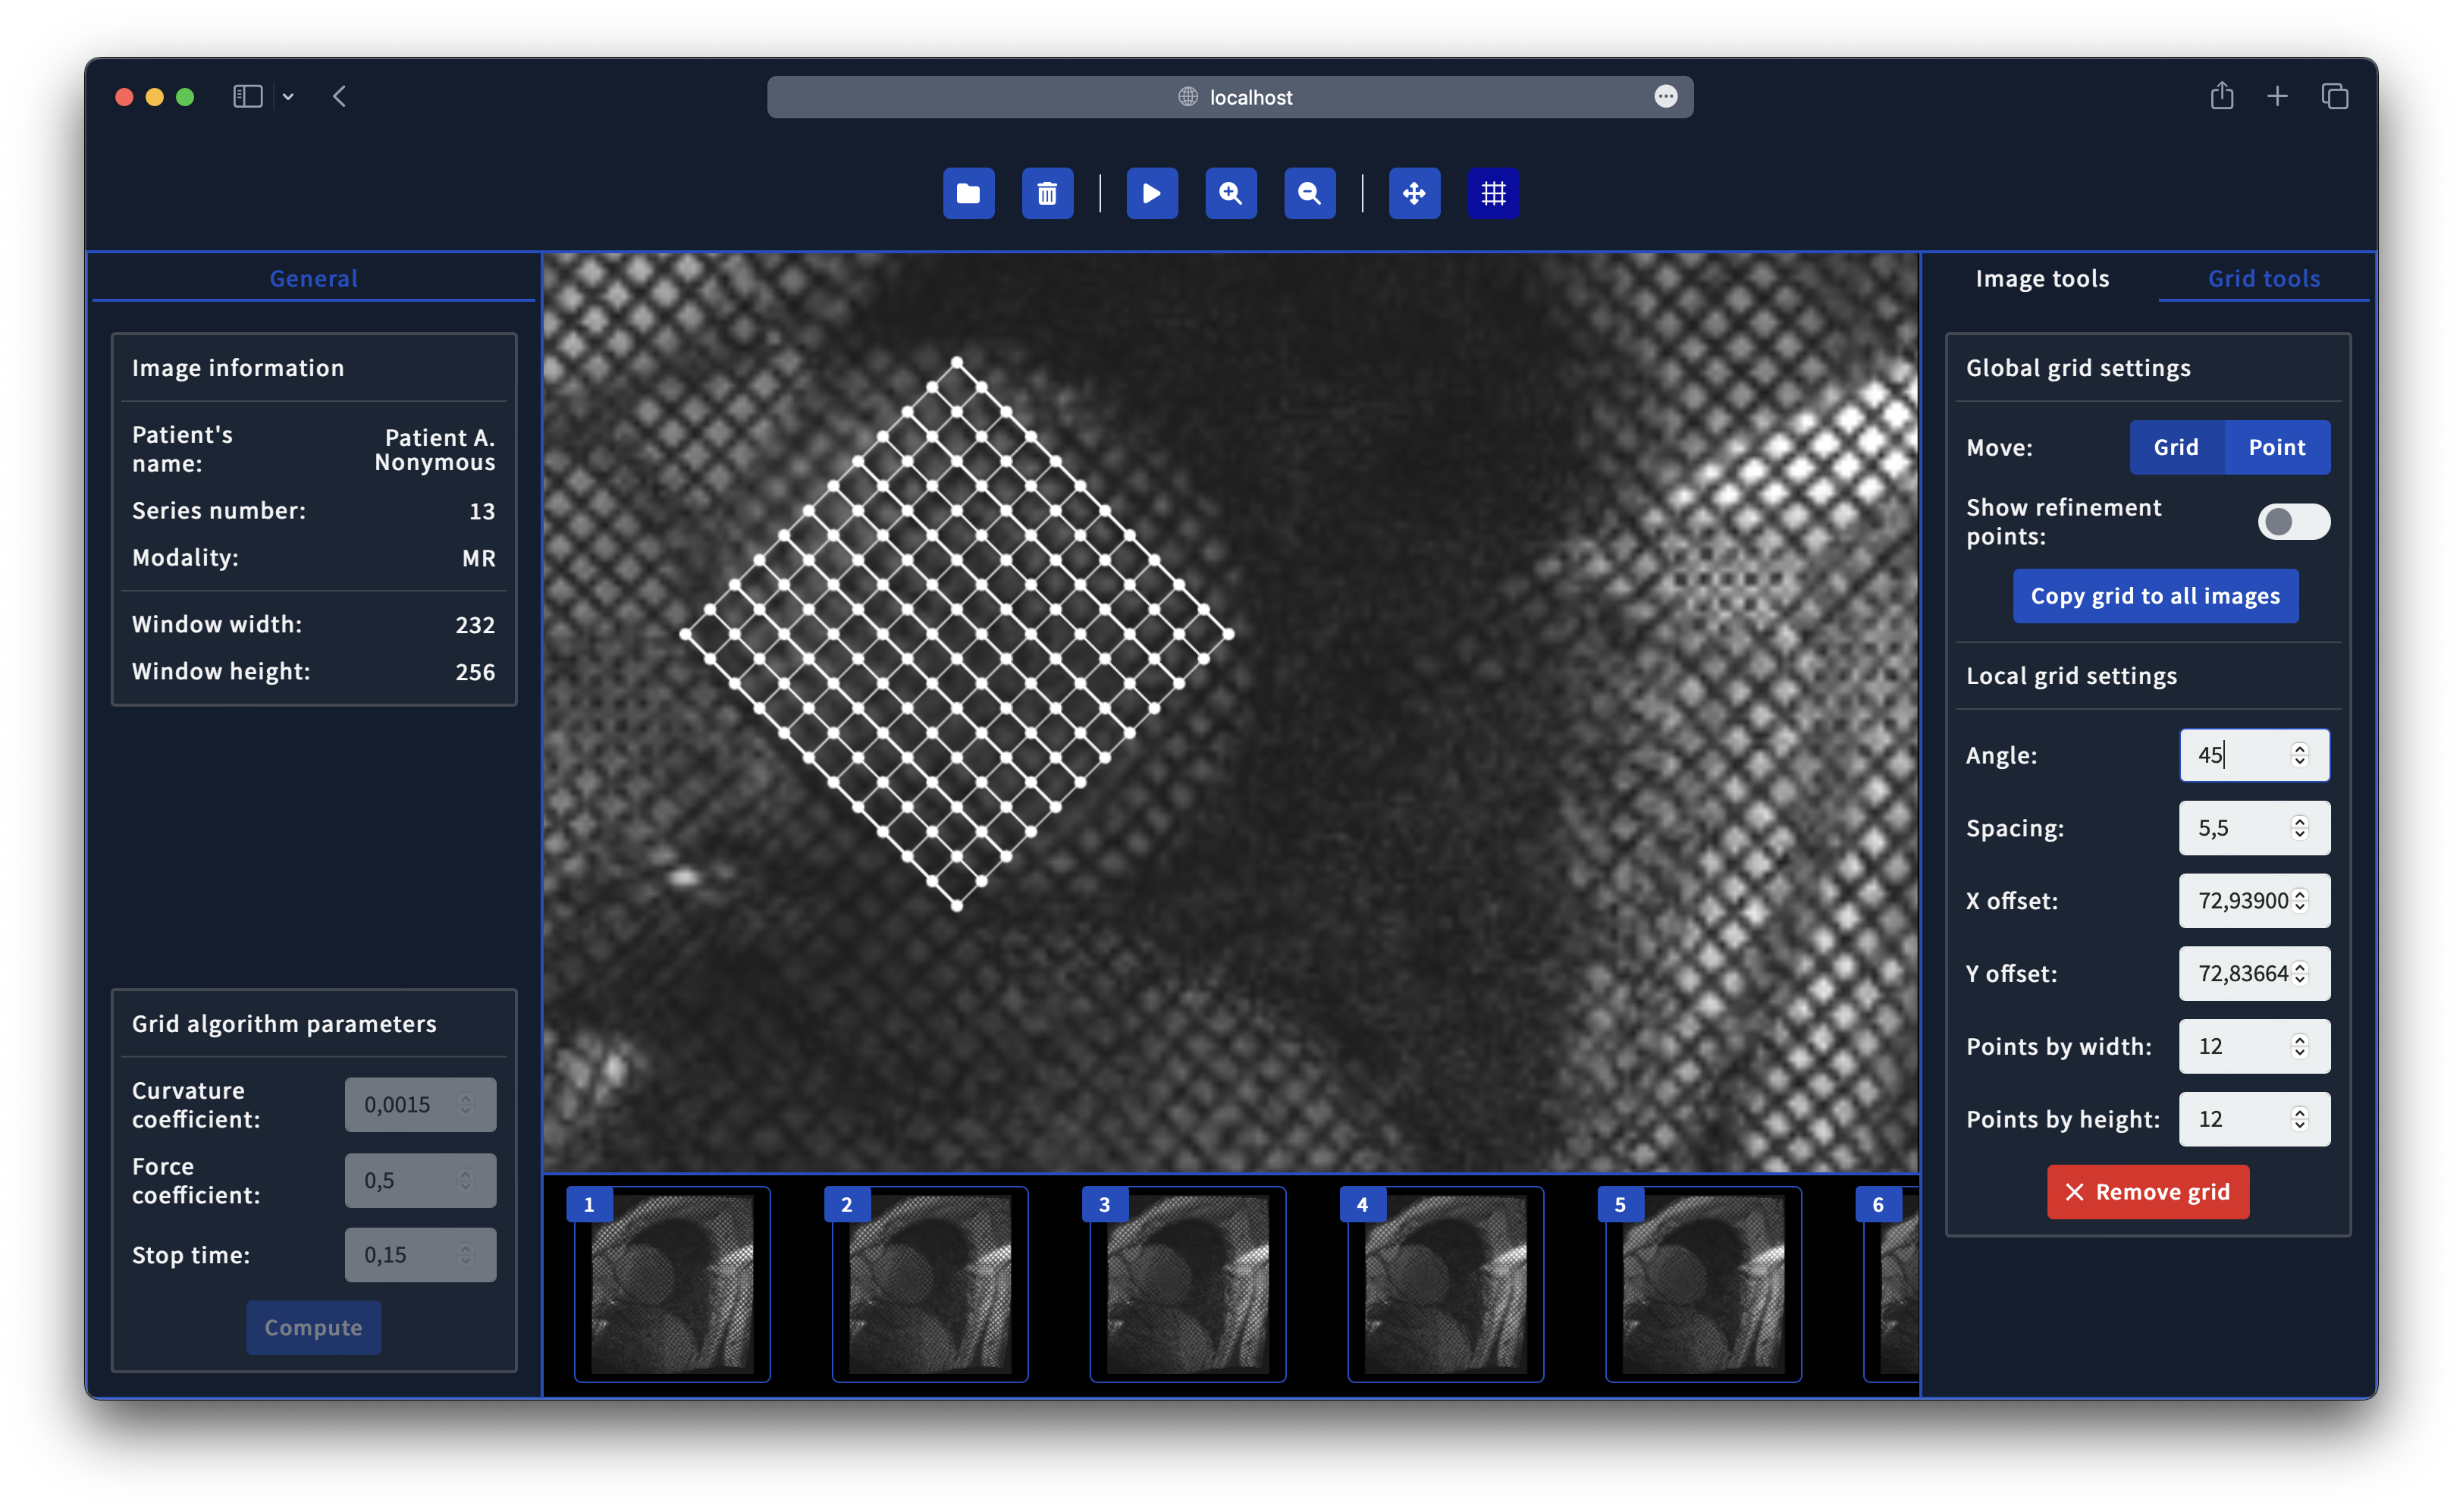
\includegraphics[height=9cm]{media/new_app/zoomed_in.png}
        \captionsetup{justification=centering}
        \captionof{figure}{Snímka zobrazujúca priblíženú DICOM snímku.}
\end {figure}

\begin {figure}[H]
        \centering
        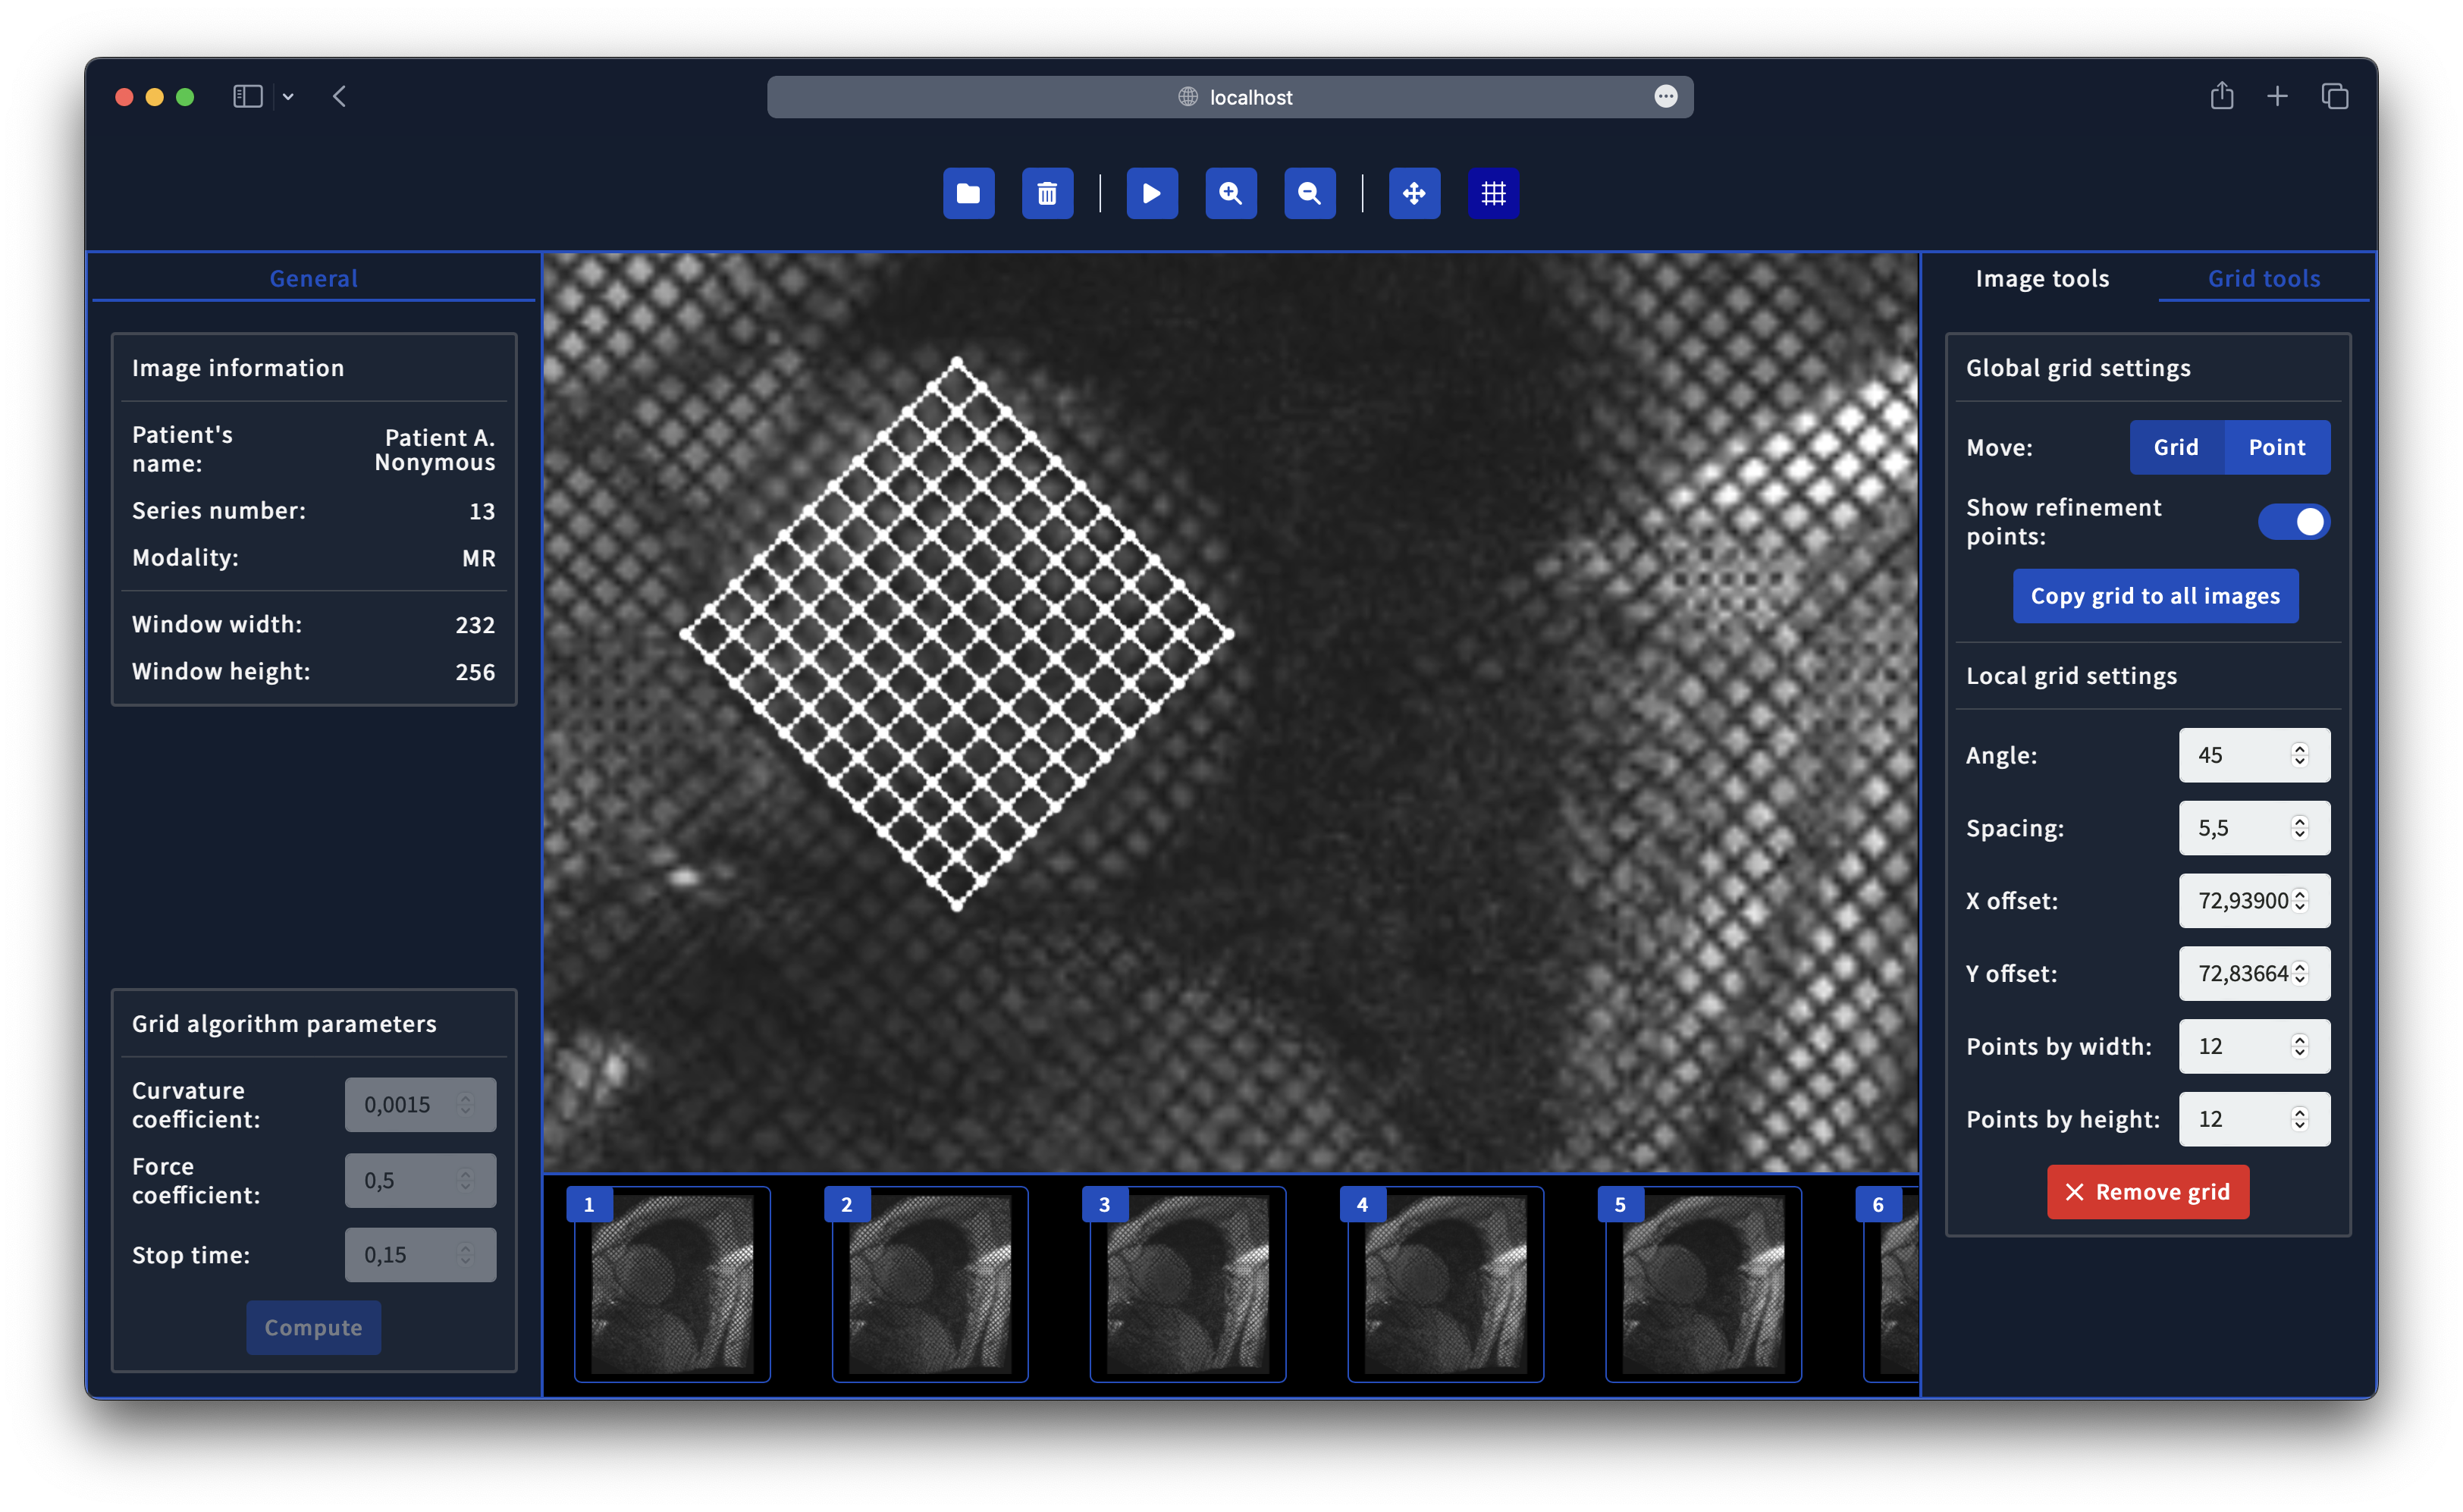
\includegraphics[height=9cm]{media/new_app/refinement_points_on.png}
        \captionsetup{justification=centering}
        \captionof{figure}{Snímka zobrazujúca \uv{refinement} body mriežky.}
\end {figure}

\begin {figure}[H]
        \centering
        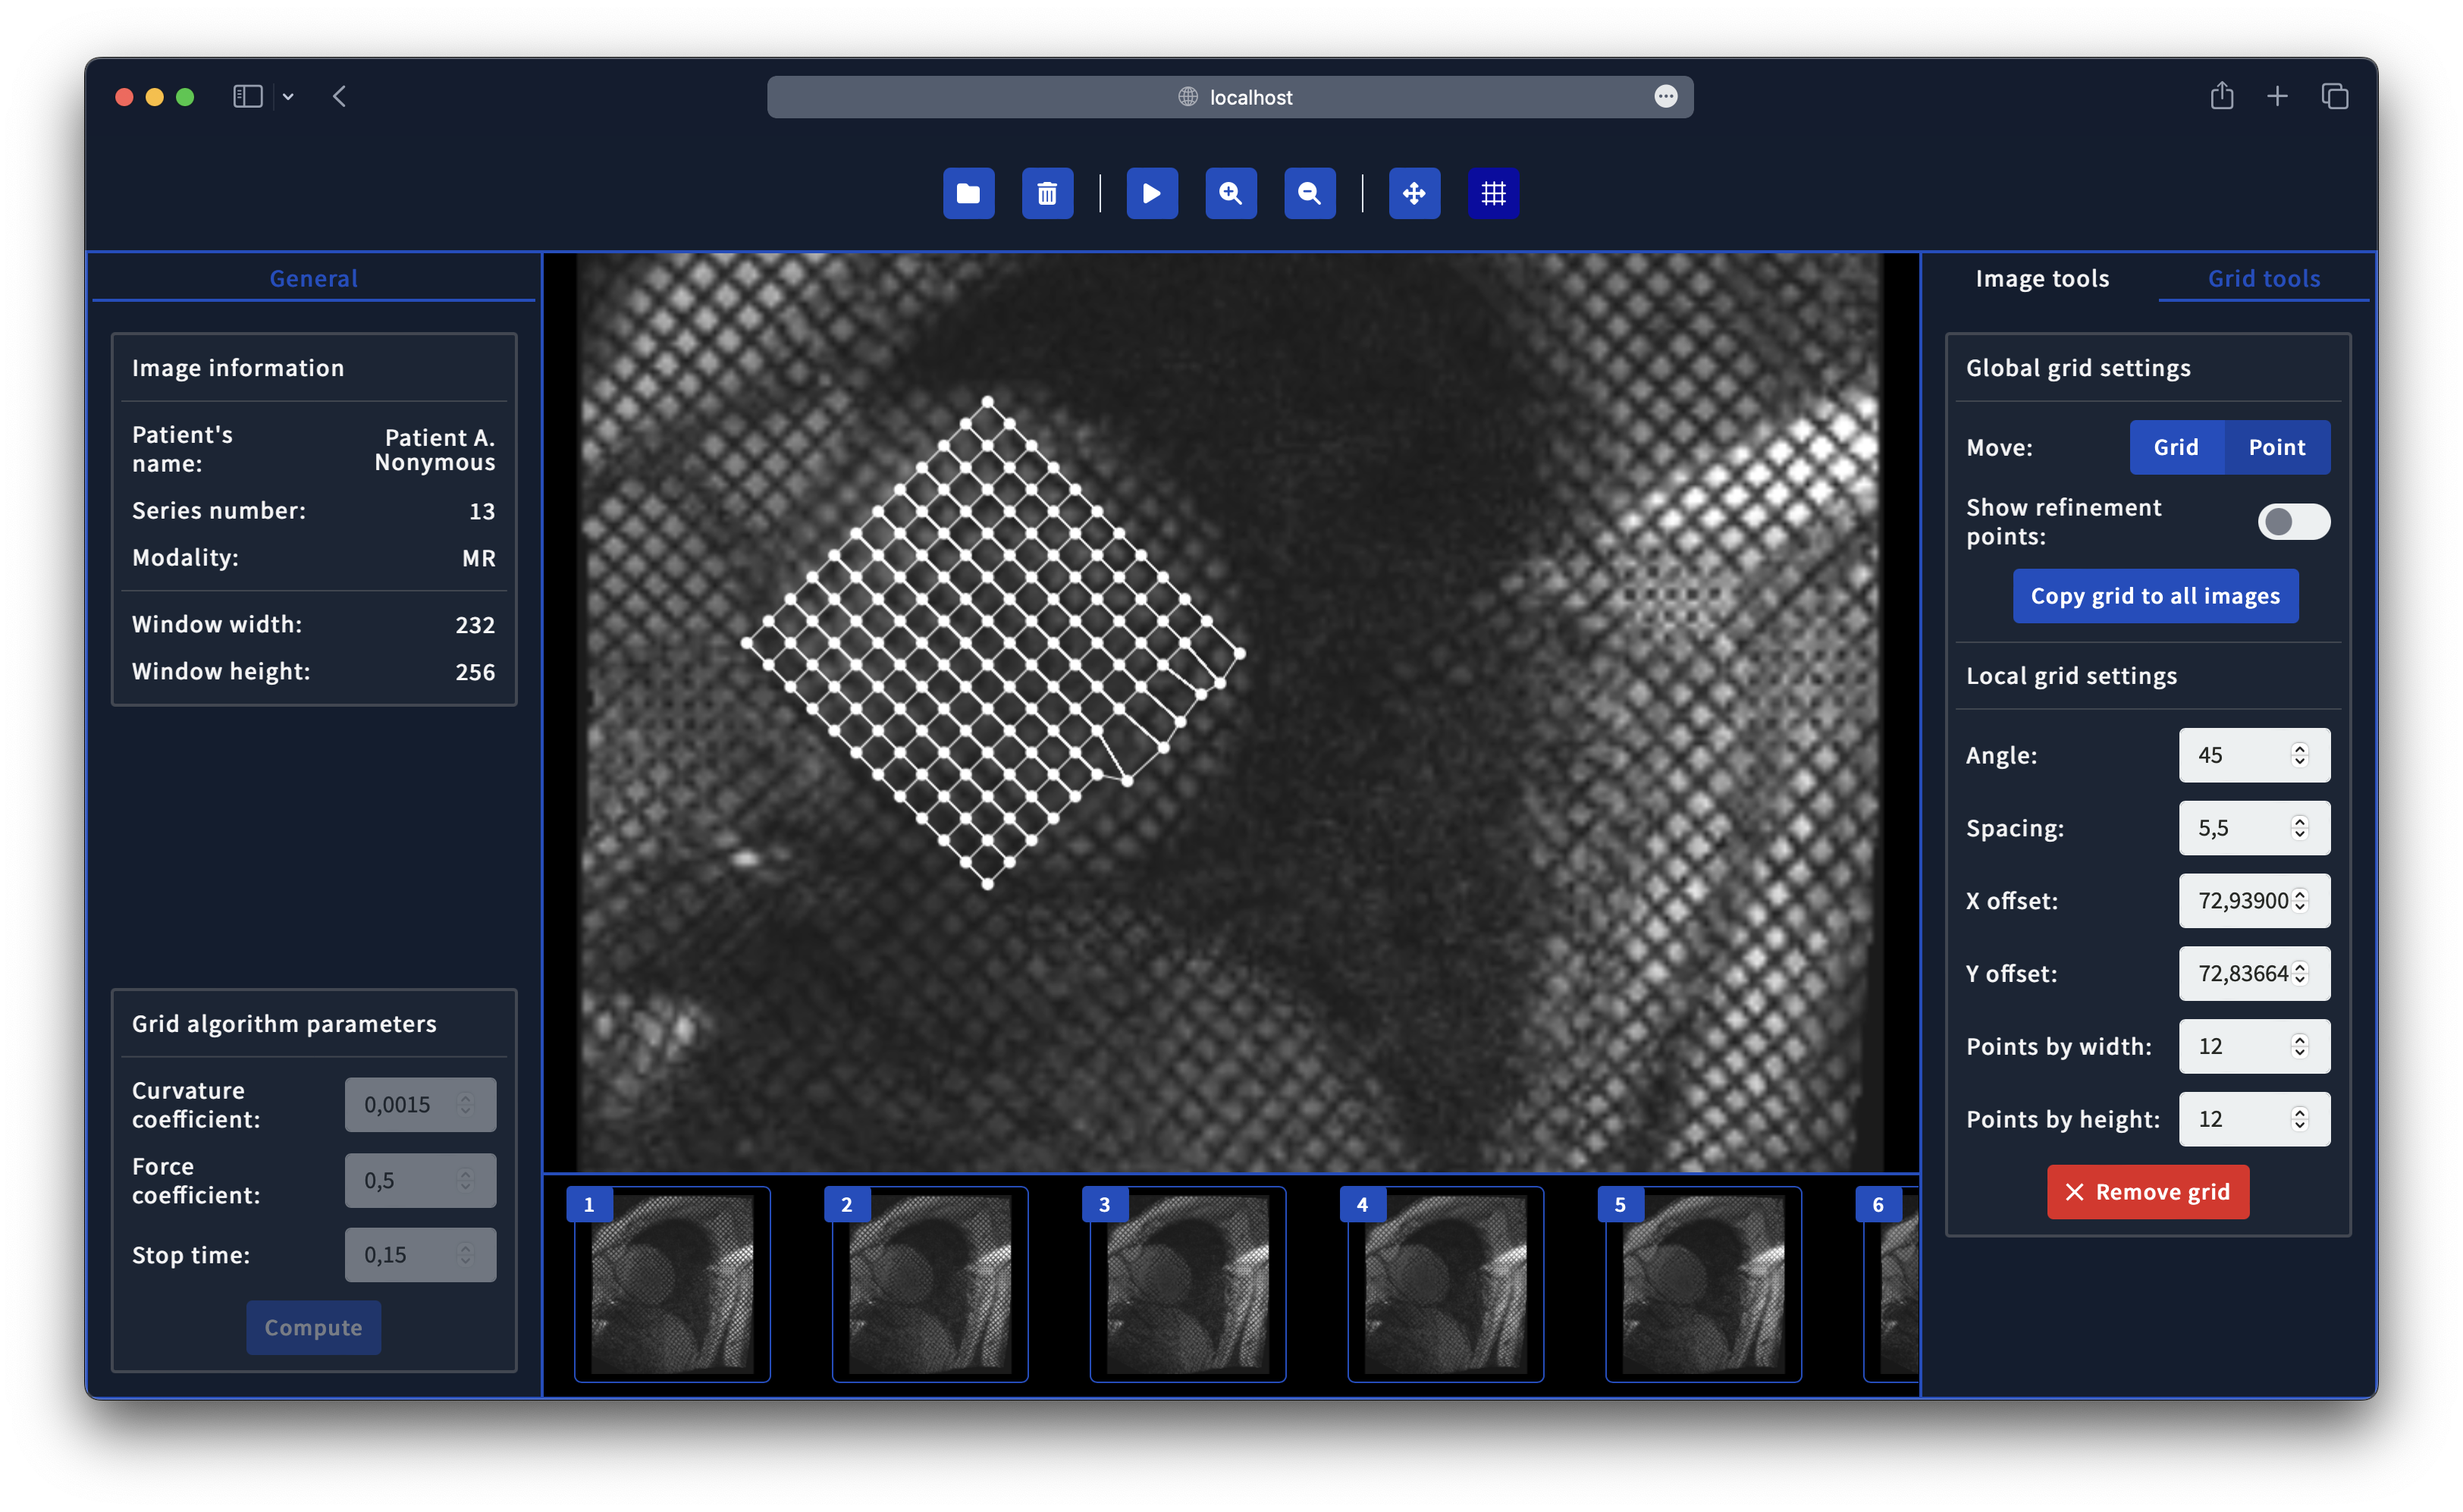
\includegraphics[height=9cm]{media/new_app/changed_points_coordinates.png}
        \captionsetup{justification=centering}
        \captionof{figure}{Snímka zobrazujúca zmenené koordináty niektorých bodov vykreslenej mriežky.}
\end {figure}

\begin {figure}[H]
        \centering
        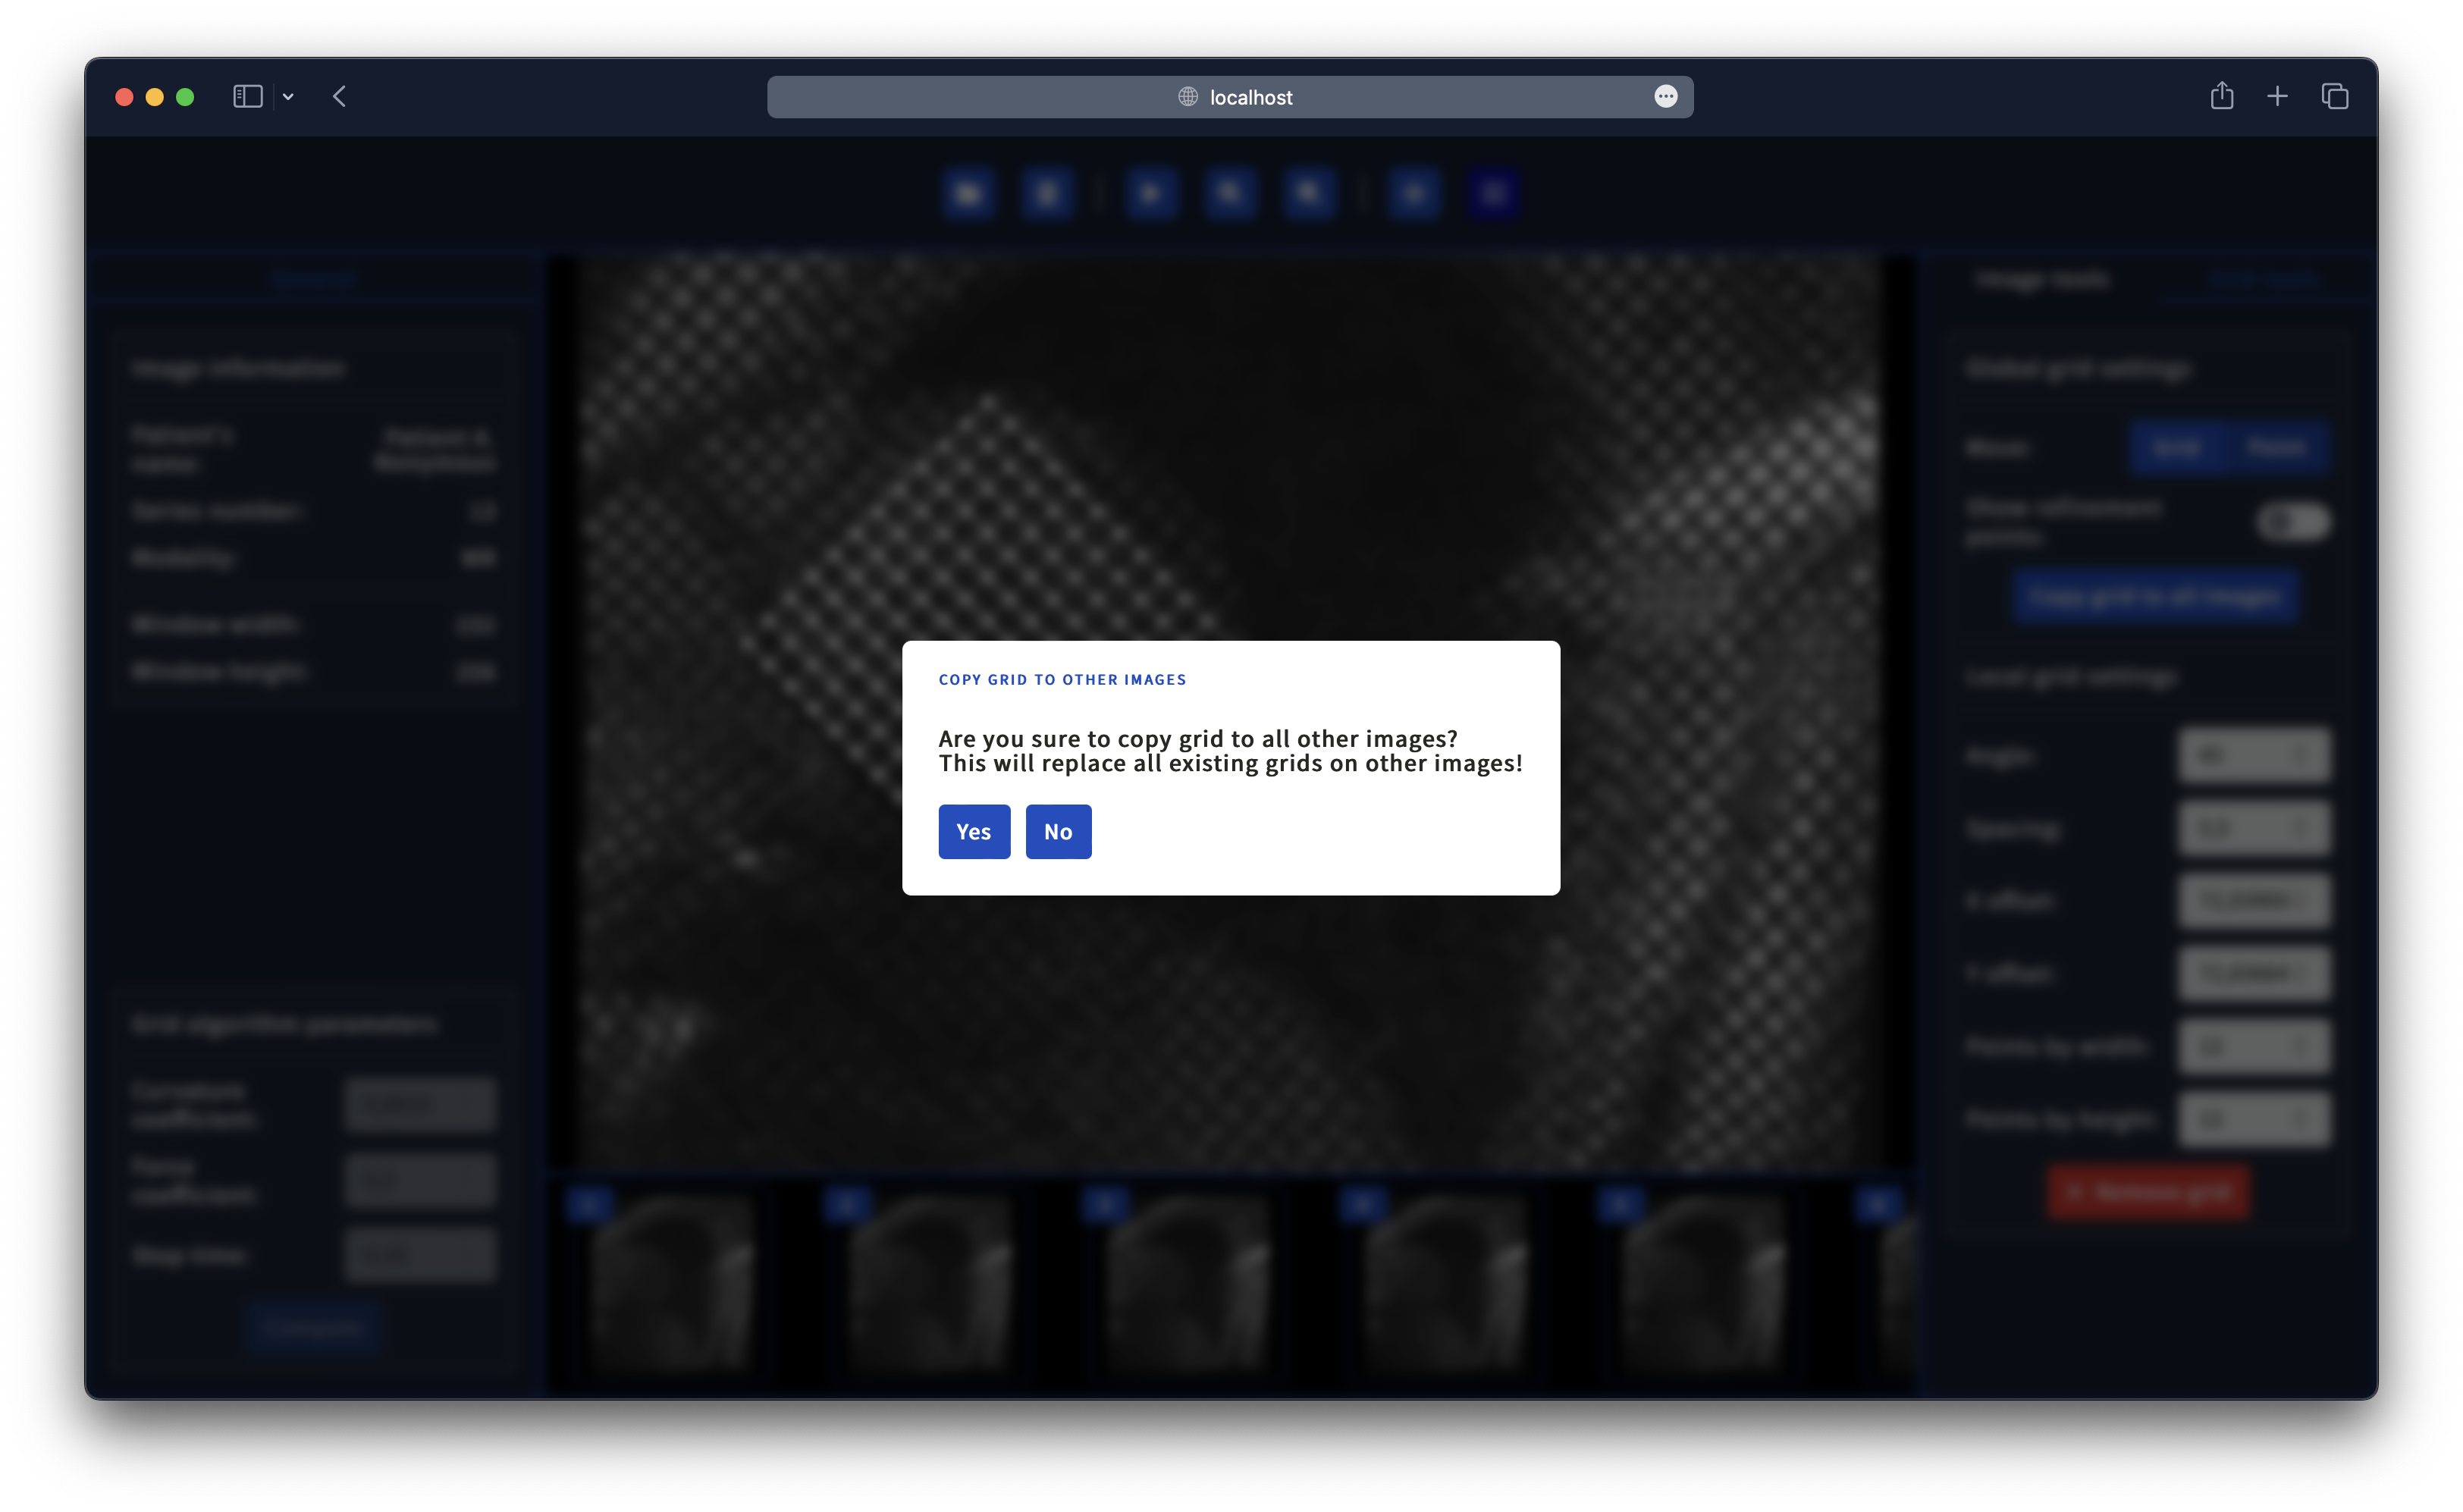
\includegraphics[height=9cm]{media/new_app/copy_grid_modal.png}
        \captionsetup{justification=centering}
        \captionof{figure}{Snímka zobrazujúca modálne okno, ktoré varuje pred prepísaním existujúcich mriežok vykreslených na ostatných DICOM snímkach, v prípade zvolenia možnosti skopírovania aktuálne zobrazenej mriežky do ostatných snímiek.}
\end {figure}